%%%%%%%%%%%%%%%%%%%%%%%%%%%%%%%%%%%%%%%%
% Compact Laboratory Book
% LaTeX Template
% Version 1.0 (4/6/12)
%
% This template has been downloaded from:
% http://www.LaTeXTemplates.com
%
% Original author:
% Joan Queralt Gil (http://phobos.xtec.cat/jqueralt) using the labbook class by
% Frank Kuster (http://www.ctan.org/tex-archive/macros/latex/contrib/labbook/)
%
% License:
% CC BY-NC-SA 3.0 (http://creativecommons.org/licenses/by-nc-sa/3.0/)
%
% Important note:
% This template requires the labbook.cls file to be in the same directory as the
% .tex file. The labbook.cls file provides the necessary structure to create the
% lab book.
%
% The \lipsum[#] commands throughout this template generate dummy text
% to fill the template out. These commands should all be removed when 
% writing lab book content.
%
% HOW TO USE THIS TEMPLATE 
% Each day in the lab consists of three main things:
%
% 1. LABDAY: The first thing to put is the \labday{} command with a date in 
% curly brackets, this will make a new section showing that you are working
% on a new day.
%
% 2. EXPERIMENT/SUBEXPERIMENT: Next you need to specify what 
% experiment(s) and subexperiment(s) you are working on with a 
% \experiment{} and \subexperiment{} commands with the experiment 
% shorthand in the curly brackets. The experiment shorthand is defined in the 
% 'DEFINITION OF EXPERIMENTS' section below, this means you can 
% say \experiment{pcr} and the actual text written to the PDF will be what 
% you set the 'pcr' experiment to be. If the experiment is a one off, you can 
% just write it in the bracket without creating a shorthand. Note: if you don't 
% want to have an experiment, just leave this out and it won't be printed.
%
% 3. CONTENT: Following the experiment is the content, i.e. what progress 
% you made on the experiment that day.
%
%%%%%%%%%%%%%%%%%%%%%%%%%%%%%%%%%%%%%%%%%

%----------------------------------------------------------------------------------------
%	PACKAGES AND OTHER DOCUMENT CONFIGURATIONS
%----------------------------------------------------------------------------------------                               

\documentclass[fontsize=11pt, % Document font size
                             paper=letter, % Document paper type
                             twoside, % Shifts odd pages to the left for easier reading when printed, can be changed to oneside
                             captions=tableheading,
                             index=totoc,
                             hyperref]{labbook}

%\documentclass[idxtotoc,hyperref,openany]{labbook} % 'openany' here removes the
   
\usepackage[bottom=10em]{geometry} % Reduces the whitespace at the bottom of the page so more text can fit

\usepackage[english]{babel} % English language
\usepackage{lipsum} % Used for inserting dummy 'Lorem ipsum' text into the template

\usepackage[utf8]{inputenc} % Uses the utf8 input encoding
\usepackage[T1]{fontenc} % Use 8-bit encoding that has 256 glyphs

\usepackage[osf]{mathpazo} % Palatino as the main font
\linespread{1.05}\selectfont % Palatino needs some extra spacing, here 5% extra
\usepackage[scaled=.88]{beramono} % Bera-Monospace
\usepackage[scaled=.86]{berasans} % Bera Sans-Serif

\usepackage{booktabs,array} % Packages for tables

\usepackage{amsmath} % For typesetting math
\usepackage{graphicx} % Required for including images
\usepackage{etoolbox}
\usepackage[norule]{footmisc} % Removes the horizontal rule from footnotes
\usepackage{lastpage} % Counts the number of pages of the document


\usepackage[dvipsnames]{xcolor}  % Allows the definition of hex colors
\definecolor{titleblue}{rgb}{0.16,0.24,0.64} % Custom color for the title on the title page
\definecolor{linkcolor}{rgb}{0,0,0.42} % Custom color for links - dark blue at the moment

\usepackage{tikz}
% load libraries
\usetikzlibrary{backgrounds,calc,patterns,decorations.pathmorphing,decorations.markings}
\usepackage[siunitx,smartlabels]{circuitikz}
\def\myGrid{1}

\addtokomafont{title}{\Huge\color{titleblue}} % Titles in custom blue color
\addtokomafont{chapter}{\color{OliveGreen}} % Lab dates in olive green
\addtokomafont{section}{\color{Sepia}} % Sections in sepia
\addtokomafont{pagehead}{\normalfont\sffamily\color{gray}} % Header text in gray and sans serif
\addtokomafont{caption}{\footnotesize\itshape} % Small italic font size for captions
\addtokomafont{captionlabel}{\upshape\bfseries} % Bold for caption labels
\addtokomafont{descriptionlabel}{\rmfamily}
\setcapwidth[r]{10cm} % Right align caption text
\setkomafont{footnote}{\sffamily} % Footnotes in sans serif

\deffootnote[4cm]{4cm}{1em}{\textsuperscript{\thefootnotemark}} % Indent footnotes to line up with text

\DeclareFixedFont{\textcap}{T1}{phv}{bx}{n}{1.5cm} % Font for main title: Helvetica 1.5 cm
\DeclareFixedFont{\textaut}{T1}{phv}{bx}{n}{0.8cm} % Font for author name: Helvetica 0.8 cm

\usepackage[nouppercase,headsepline]{scrpage2} % Provides headers and footers configuration
\pagestyle{scrheadings} % Print the headers and footers on all pages
\clearscrheadfoot % Clean old definitions if they exist

\automark[chapter]{chapter}
\ohead{\headmark} % Prints outer header

\setlength{\headheight}{25pt} % Makes the header take up a bit of extra space for aesthetics
\setheadsepline{.4pt} % Creates a thin rule under the header
\addtokomafont{headsepline}{\color{lightgray}} % Colors the rule under the header light gray

\ofoot[\normalfont\normalcolor{\thepage\ |\  \pageref{LastPage}}]{\normalfont\normalcolor{\thepage\ |\  \pageref{LastPage}}} % Creates an outer footer of: "current page | total pages"

% These lines make it so each new lab day directly follows the previous one i.e. does not start on a new page - comment them out to separate lab days on new pages
\makeatletter
\patchcmd{\addchap}{\if@openright\cleardoublepage\else\clearpage\fi}{\par}{}{}
\makeatother
\renewcommand*{\chapterpagestyle}{scrheadings}

% These lines make it so every figure and equation in the document is numbered consecutively rather than restarting at 1 for each lab day - comment them out to remove this behavior
\usepackage{chngcntr}
\counterwithout{figure}{labday}
\counterwithout{equation}{labday}

% Hyperlink configuration
\usepackage[
    pdfauthor={}, % Your name for the author field in the PDF
    pdftitle={Laboratory Journal}, % PDF title
    pdfsubject={}, % PDF subject
    bookmarksopen=true,
    linktocpage=true,
    urlcolor=linkcolor, % Color of URLs
    citecolor=linkcolor, % Color of citations
    linkcolor=linkcolor, % Color of links to other pages/figures
    backref=page,
    pdfpagelabels=true,
    plainpages=false,
    colorlinks=true, % Turn off all coloring by changing this to false
    bookmarks=true,
    pdfview=FitB]{hyperref}

\usepackage[stretch=10]{microtype} % Slightly tweak font spacing for aesthetics

\usepackage{mdframed}
\usepackage{todonotes}
\usepackage{epstopdf}
\epstopdfsetup{suffix={}}
%\setlength\parindent{0pt} % Uncomment to remove all indentation from paragraphs


\usepackage{minted}
\usepackage{mdframed}


%----------------------------------------------------------------------------------------
%	DEFINITION OF EXPERIMENTS
%----------------------------------------------------------------------------------------

% Template: \newexperiment{<abbrev>}[<short form>]{<long form>}
% <abbrev> is the reference to use later in the .tex file in \experiment{}, the <short form> is only used in the table of contents and running title - it is optional, <long form> is what is printed in the lab book itself

\newexperiment{example}[Example experiment]{This is an example experiment}
\newexperiment{example2}[Example experiment 2]{This is another example experiment}
\newexperiment{example3}[Example experiment 3]{This is yet another example experiment}

\newsubexperiment{subexp_example}[Example sub-experiment]{This is an example sub-experiment}
\newsubexperiment{subexp_example2}[Example sub-experiment 2]{This is another example sub-experiment}
\newsubexperiment{subexp_example3}[Example sub-experiment 3]{This is yet another example sub-experiment}

%----------------------------------------------------------------------------------------
\newcommand{\HRule}{\rule{\linewidth}{0.5mm}} % Command to make the lines in the title page

\setlength\parindent{0pt} % Removes all indentation from paragraphs

\begin{document}

%----------------------------------------------------------------------------------------
%	TITLE PAGE
%----------------------------------------------------------------------------------------
%\frontmatter % Use Roman numerals for page numbers

%\begin{center}

%

\title{
\begin{center}
\href{http://www.bradley.edu}{
\includegraphics[height=0.5in]{figs/logoBU1-Print}}
\vskip10pt
\HRule \\[0.4cm]
{\Huge \bfseries Laboratory Notebook \\[0.5cm] \Large BEMOSS: }\\[0.4cm] % Degree
\HRule \\[1.5cm]
\end{center}
}
\author{\Huge R. Bachman \and \Huge J. Ingram  \and \Huge R. O'Malley \\ \\ \LARGE bemoss2019@gmail.com \\[2cm]} % Your name and email address
\date{Beginning September 2018} % Beginning date
\maketitle

%\maketitle % Title page

\printindex
\tableofcontents % Table of contents
\newpage % Start lab look on a new page

\begin{addmargin}[0cm]{0cm} % Makes the text width much shorter for a compact look

\pagestyle{scrheadings} % Begin using headers

%----------------------------------------------------------------------------------------
%	LAB BOOK CONTENTS
%----------------------------------------------------------------------------------------

\labday{Tuesday, 8 May 2018}


Today we had our first meeting with everyone attending. We discussed what we were going to do over the summer and decided that we will be planning on working with some of the simpler examples first and then continuing onto the harder ones after.

\labday{Monday, 14 May 2018}
Robert \newline 
Today I read through the documents provided to us and thought of one of the first things to do which is simply work with the smart plug which is explained in the documents, then use the IFTTT to simply send and email or text if the load has been unplugged. This is just to get a basic understanding of how everything works in these situations and should be a good starting point for the rest of the project,.
%-----------------------------------------

\experiment{example}

Write about experiment..


%-----------------------------------------

\subexperiment{subexp_example}

Write about subexperiment. 
%-----------------------------------------

%----------------------------------------------------------------------------------------
 
\end{addmargin}

\labday{Monday, 21 May 2018}
Today Reece researched the hierarchy of BEMOSS software. According to the BEMOSS developer resources, the hierarchy consists of 4 layers. Starting at the top, level 1 is a practical user inferface (UI) which offers the ability to track and control loads, depending on clearance settings. Apache Cassandra is employed in layer 2, called "Application and Data Management". A few aspects of this layer may be neat to apply to our project such as planning/ scheduling and behavior pattern analysis. Layer 3 is the operating system and framework. VOLTTRON, developed by NPPL, is the software platform that BEMOSS is  built on. Here, email and SMS notifications are produced and detection of IoT devices is undergone and their APIs determined. Layer 4 is called the connectivity layer. The BEMOSS foundation describes this as a translation layer as this layer translates between the BEMOSS commands to various devices without knowing their individual API. 

\labday{Tuesday, 29 May 2018}
Robert \newline
I attempted to install BEMOSS onto my laptop today and came up with a few problems in my situation. The first was when attmepting to install after downloading which comes from running the startBEMOSS GUI.sh. This problem gave me an output from ImageTk which I did not know the whereabouts of. After reading through the start bemoss script I found out it ran the GUI.py, all of which can be found at github.com/bemoss/BEMOSS3.5. This script was attempting to import ImageTk which was giving issues and from looking at the line just above it I recognized that there might be a problem due to the differences in python 2 and 3. The line above wrote from PIL import Image, so there could be a problem there and that solved the first problem, allowing the GUI to run properly. After the GUI started to run I was able to install BEMOSS and went through the installation process found at github.com/bemoss/BEMOSS3.5/wiki. From that point I restarted my virtual machine and attempted to run BEMOSS but at the end of trying to run BEMOSS I am given an error "'gevent event AsyncResult' object has no attribute 'ident'". This made me think that I had done something wrong so I restarted the process and re installed BEMOSS which gave me the same error. Upon further research I have come to realize that there is a problem with gevent which has just recently been updated which makes BEMOSS not work anymore. To fix this we would need to remove our current gevent package and change it with version 1.2.2 to possibly have BEMOSS work. This is not a surefire solution since we do not know what else has changed since then.
\labday{Saturday, 2 May 2018}
Robert \newline
I again attempted to install BEMOSS onto my laptop today and had the same problems. I went through most of the packages that are required like the gevent that was supposed to be updated very recently and I was still not able to get BEMOSS to work. After the update gevent version was supposed to be version 1.2.2 which was supposed to fix the problem. When checking the version It did come up as version 1.2.2 but that did not fix the issue. After starting BEMOSS I get an error of 'ImportError: No module named netifaces'. After checking the version I was able to find that I did have the netifaces package installed properly and now am wondering where my issue is coming in. There is also an issue saying there is no setup.py which does exist in the unzipped folder but is not in the GUI folder. I am wondering if python is allowing packages to be used in all situations or if it is limiting access in which case I will need to find a way to fix that issue. I am also wondering if everything is configured properly for a new update for python since ImageTk had to be changed from import ImageTk to from PIL import ImageTK. n
\labday{Monday, 11 June 2018}
Jordan \newline
I reinstalled the BEMOSS software today before our meeting with the BEMOSS technician which resulted in my BEMOSS running. During the meeting it was discovered that the current issue that Robert and Reece had was due to using xubuntu 18.04 rather than 16.04. Robert installed ubuntu 16.04 before the meeting. While installing BEMOSS on the new virtualbox he ran into another problem as his laptop could not connect to ubuntu's servers. After this issue he began to reinstall a brand new virtualbox, this issue persisted however. The meeting ended with Robert and Reece still without a running version of BEMOSS however Robert will install a new version of ubuntu and try again. Another meeting will be held June 12 at 5:00pm.
\labday{Thursday, 5 July 2018}
Robert \newline
Today I reinstalled BEMOSS. I did not go from a fresh machine but the only thing that needs to happen there is to install the correct version of ubuntu which has to be version 16.04 as documented in their help guide. I started by opening a command terminal and typing sudo apt-get update then sudo apt-get upgrade to make sure that everything else that I have installed on the machine is up to date and will not cause problems for the rest of the software. After doing that I ran the command %
%
\begin{verbatim}
dpkg --get-selections    
\end{verbatim}
%
and  looked for git. In my case it showed up but if not I would have typed %
%
\begin{verbatim}
sudo apt-get install git     
\end{verbatim}
%
to install the software that is necessary to download BEMOSS. Once I verify that I have git, I type %
%
\begin{verbatim}
  git clone -b master https://github.com/bemoss/BEMOSS3.5.git  
\end{verbatim}
%   
  so that I download all of the software for BEMOSS from github. Once everything is downloaded I go into the newly downloaded BEMOSS directory that should be in my home directory and enter the GUI directory. I then type 
  %
  \begin{verbatim}
  ./startBEMOSS GUI.sh    
  \end{verbatim}
  %
  so enable the GUI for BEMOSS. After clicking run BEMOSS the program will prompt me if I would like to install BEMOSS as it has not yet been installed so I click yes and wait for some of the questions that the software will have for me. I respond to the prompts with whatever response I want and then go onto the post installation process. To start out I go to advanced settings in the BEMOSS GUI and go to database Configuration files to change a few of things that I nned to in order to get this to work. i then change line 59 in postgresql.conf from \#listen addresses = 'localhost' \# what IP address(es) to listen on; to listen addresses = '*' \# what IP address(es) to listen on; as well as line 82 on pg hba.conf: from %
%  
\begin{verbatim}
host    all     all     127.0.0.1/32
to 
host    all     all     127.0.0.1/32        md5
host    all     all     10.0.2.15/32        md5     
\end{verbatim}
%
where 10.0.2.15 is my specific ip address. After that I still have to go to multinode \emph{data.json} and modify the line with \emph{"address": tcp://192.168.10.62:9000"} so that it read \emph{"address": tcp://10.0.2.15:9000} where the numbers that I changed again were changed because that is what my ip address is. After that I made sure I saved everything and clicked run BEMOSS again and it worked.


\labday{Thursday Aug. 02, 2018}
Dr. Miah

Last couple of weeks, I have been researching on how to make efficient use of BEMOSS and what could be our original contributions. I read couple of papers on smart grid (see~\cite{Mocanu2018,Mocanu2018,FrancoisLavet2014,FrancoisLavet2017}) and building energy management (see~\cite{Ferreira2012,Pipattanasomporn2015,Khamphanchai2015,Zhang2016}).  


\labday{Monday, 11 June 2018}
Reece \newline
Throughout the summer, I have been working on a personal project involving control of a DC motor through Alexa. Through doing this, I have extensively researched a dual H bridge module called L298N. H-Bridges allow for a controlled polarity change via transistors and diodes to reverse the direction of a motor. The 298N has 2 H-bridges which can control 2 DC motors or 1 bipolar stepper motor (due to steppers having phases). \newline
\newline The L298N has various pin controlled functions which will be very useful for our application. The L298N has PWM capabilities for each channel, thus controlling the speed of each DC motor separately. 
\newline\newline The module's power supply portion has a few functions that may be of interest to us if we want to make a compact, final product. The module can control motors that operate between 5 and 35V DC. The module's logic runs at 5V so a convenient on-board 5V regulator is provided. This regulator is only to be used with input voltages up to 12V. In my experience, the board and heat sink run very hot when supplying 12V, so I would recommend using something smaller. When the on-board 5V regulator is enabled (via a jumper), a 5V power supply becomes available to an external circuit. This 5V power supply can be very useful to power our RPI or other controller if we would like to keep our circuit efficient and run only 1 power supply. Precautions may need to be taken to protect the circuit being supplied the 5V in the case of a power surge on the motor end. When a motor is to be ran at voltage greater than 12V, the 5V regulator jumper must be removed and motor power supplied in the 12V port with 5V applied to the 5V port for the module logic. In my experience, the 5V regulator runs the risk of causing "Brown Out" issues if not careful. Brown out occurs when a spike of high power demand occurs and the power supply does not supply enough to keep up. In my experience, when my stepper motor was under load, it drew too much power and fried the module to failure. After further research, I found the 5V regulator consumes about 1.4V which I did not account for. I found the safest-case scenario is when separate motor and 5V logic power supplies are available to the module. This will allow for a power supply to directly supply all of it's power to the motors and not get diluted in the regulation process. This safety method may be removed after prototyping or thorough calculations including motor and board requirements have been made. 
\newline\newline
Next to the power supply ports are the function control pins. The board has 4 pins dedicated to switching the 4 H-bridge transistors on and off. On the outer side of these 4 transistor control pins are the ENA and ENB pins which allow for PWM control of respective channels. If the jumper is removed and a wire with PWM control added, PWM mode is enabled. If the jumper is in place, the respective motor channel is running on the full power supplied by the power supply. 


\labday{Friday, 24 August 2018}
The group met 3-4 today. We further discussed the group workload and agreed on the following: Reece is in charge of the hardware, interfacing and libraries. Bob is in charge of knowing BEMOSS workings and code inside and out and will create the script to control the hardware created by Reece. Jordan will conduct research to develop an algorithm to implement in BEMOSS to allow BEMOSS to automate a building. 
\newline The group will have weekly meetings on Fridays at 3pm and will meet in the lab Tuesdays and Thursdays 3:30-6:30. 

\labday{Tuesday, 28 August 2018}
The group met for the first day in the lab. Bob successfully set up the BEMOSS server on his laptop, however the Wemo Wi-Fi smart plug we had ordered was not BEMOSS compatible. The documentation on the WeMo plug was not sufficient enough to conclude which versions of the WeMo plug are compatible. Next, we connected the Philips Hue smart light to a lamp, but the Philips Hue requires a Philips Hue bridge to connect to the Wi-Fi network. Reece started to compile parts list and acquire hardware that is lying around the building. We will be using a L298N dual H-bridge, 24V Pittman DC motor, and 24V power supply. Reece made a high-level flow chart detailing the command flow from the user's laptop to the motor. Reece started making a Orcad model of our proposed circuit.
\newline Jordan looked at the research paper by François-Lavet. He downloaded the code available on the example github page on deep reinforcement learning neural networks and was able to successfully get the code running on Robert's laptop.
\todo[inline]{Great. Reece: Include the orcad model and the flowchart here.}

\labday{Thursday, 30 August 2018}
The group met today for 3 hours in the lab. Reece familiarized himself with the powerful Ipe software which makes flowcharts and diagrams. With this, he made an overview of our BEMOSS system flow of information and instructions. 
\newline We obtained a Raspberry Pi starter kit today. The kit claims to contain a micro-SD card that has Raspbian preloaded on it. We are working on obtaining a monitor that has an HDMI port on it which will allow us to interface with the RPI directly and conveniently. Raspbian has GPIO capabilities already installed and has multiple built in Python IDE which Reece plans to program directly onto. Bob attempted to connect the raspberry pi to his laptop but we do not have serial connections to connect with putty nor do we have a monitor that can connect to the raspberry pi via hdmi. We will be able to continue with that once we get a monitor that works. Jordan was researching the paper more. In the process, he installed the DeeR (deep reinforcement) library on python. This has allowed him to start testing with the example scripts and familiarize himself with the library. This has allowed him to find out what it is that he will be doing in the future and everything that he will have to learn.

\labday{Tuesday, 4 September 2018}
Today we wrote some scripts in python for the Raspberry Pi as well as tested some new strategies for getting BEMOSS to work with the WeMo switch. Finally, Reece confirmed the compatibility of the Raspberry Pi GPIO pins to the H bridge as well as determined the logic to make the H-Bridge operate. The H-Bridge is wired to the motor and ready to take commands from the Pi.
Jordan, while understanding the python code, developed a python script to test the GPIO pin so that we can actuall yunderstand what it is that we are doing.

\labday{Thursday, 6 September 2018}
We successfully connected the motor, Raspberry Pi, and the H-bridge together and created a python test script to control the direction and speed of the motor. This test script has functioning code that initializes all of our GPIO pins, libraries, timers, and motor direction changes- so it will be a very useful reference for our future work. We created a plan to create a permanent board to mount the current hardware. This will create a better test environment that looks more professional and reduces the amount of time spent setting up the hardware each day. Robert contacted Ashraful again through email, asking for more advice on connecting the WeMo Switch to BEMOSS as we still cannot connect the switch to BEMOSS.

\labday{Friday, 7 September 2018}
Reece: Today we have a meeting with Professor miah. To start we are giving a rundown of what has been done so far. We currently have an open loop control with our motor. In the future we are looking at creating a feedback loop with the motor. Create a block diagram with all the part numbers describing what it is we have done. In the future we will be looking to make the connection from the pi to the motor driver wireless so that when using BEMOSS instead of the pi it will be much easier.
\newline Bob: We are going to try to get BEMOSS to be able to find the motor that we have currently. Our BEMOSS has come to a standstill because BEMOSS is not able to discover the WeMo switch. Send an email to Ashraf with 3 bullet points. 1 send a link for what device you are using. (ours is not working) 2 what BEMOSS version are you using, we want to replicate what you are doing. 3 link of the Philips bridge so we can try to work with that as well. 


\begin{itemize}
    \item interface wireless from pi to bridge 
    \item send an email to Ashraf, send a link for WeMo, what bemoss version, link of philips bridge 
    \item finish up the 5 papers
    \item create a block diagram for our project
    \item get ready to submit problem statement 
\end{itemize}
The top figure on the image below is a schematic of our current working motor driver set up. The figure on the bottom of the image is our plan to replace the physical connection between the Raspberry PI and the motor driver with a XBee set up. A network of XBee modules would allow for a scale-able product that could allow for countless nodes and motors to be controlled. 
\begin{figure}
  \centering
  \boxed{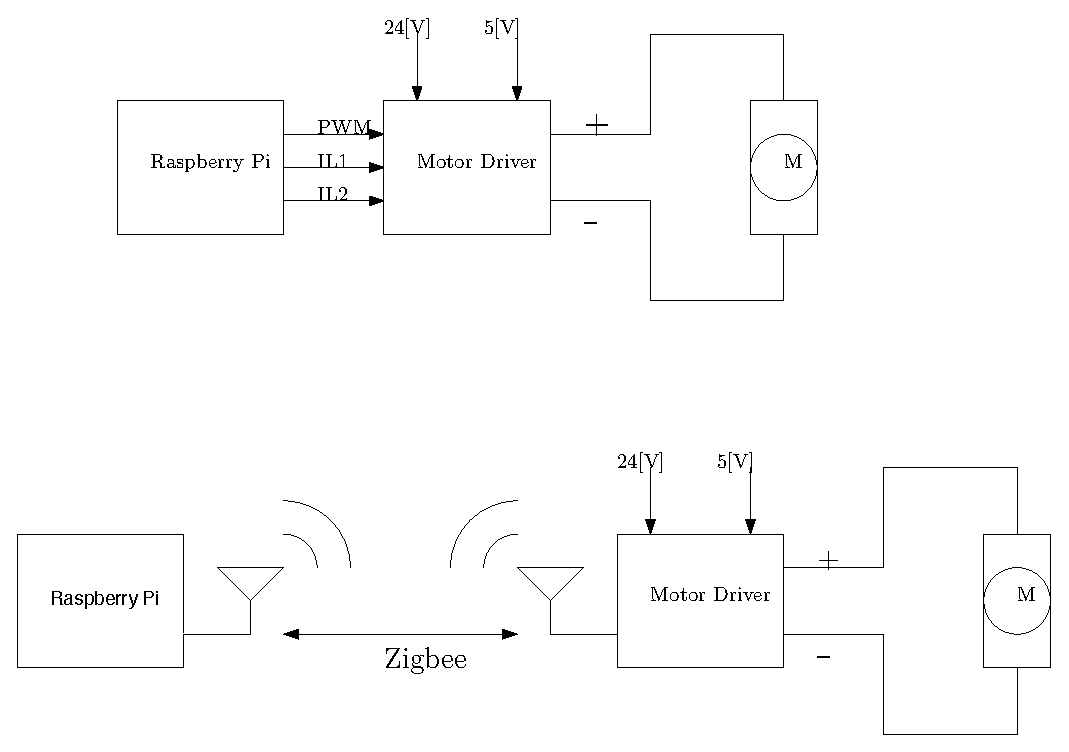
\includegraphics[width=0.5\textwidth]{figs/ipe/RpiMDInterface}}
  \caption{Raspberry Pi-Motor Driver Interface}
  \label{fig:RpiMDInterface}
\end{figure}



\begin{figure}
  \centering
  \boxed{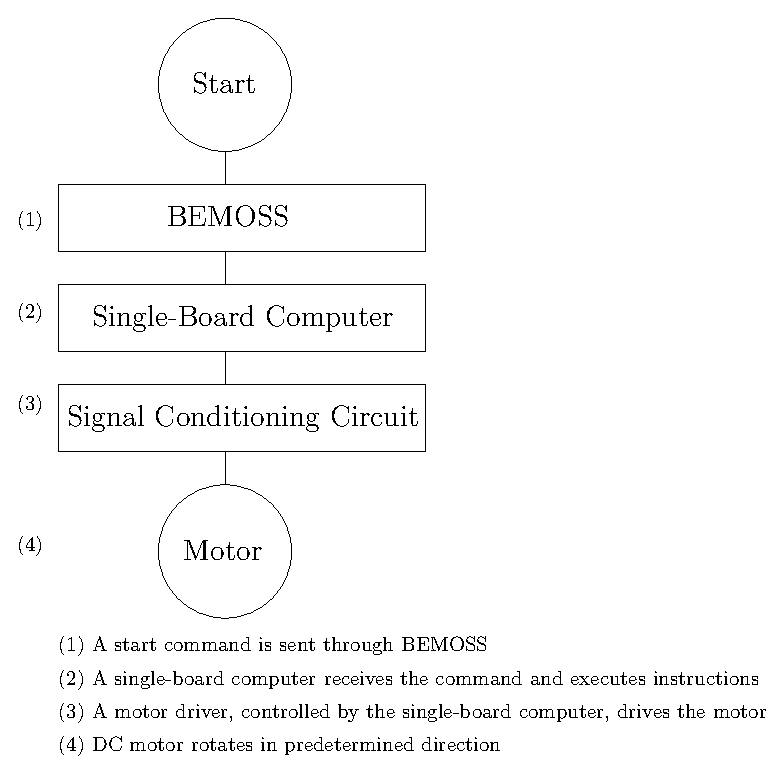
\includegraphics[width=0.5\textwidth]{figs/ipe/flowOfOperation}}
  \caption{Flow of operation of the proposed BEMOSS architecture.}
  \label{fig:flowOfOperation}
\end{figure}

\labday{September 4, 2018}
\begin{figure}
  \centering
  \boxed{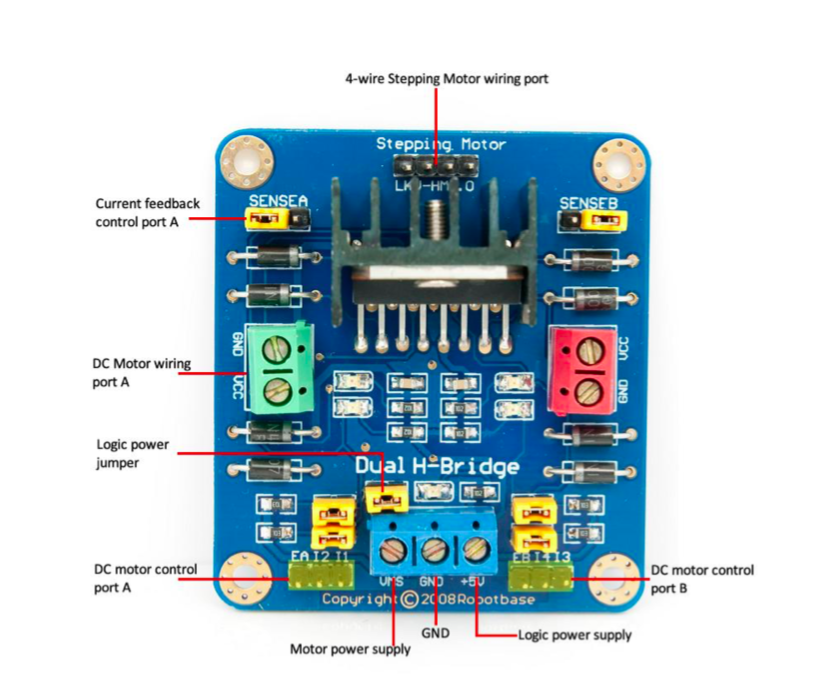
\includegraphics[width=1\textwidth]{figs/img/L298NSchematic}}
  \caption{L298N Dual H Bridge Schematic.}
  \label{fig:L298NSchematic}
\end{figure}

\begin{figure}
  \centering
  \boxed{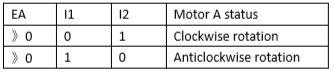
\includegraphics[width=.75\textwidth]{figs/img/PinConfigL298N}}
  \caption{L298N Pin Configuration Vs Motor Direction.}
  \label{fig:PinConfigL298N}
\end{figure}





\labday{Friday, 31 August 2018}
Today we are having our first official meeting of the semester for our senior project. To start we will define our project. For the moment we need to create a high level diagram for our project. To help build the diagram we should read some IEEE papers in order to get a better understanding of how we should create our diagram. 5-6 papers worth of system architecture should be read. Jordan should do the following: go to IEEE and write building energy management and look at at least 5 journal papers from building energy management literature and read their high level architecture and see what people have done. If there are papers that Jordan want's to read then he can contact Miah about the paper that he wants to read and he will get him the paper somehow. In the introduction section of the paperBEMOSS-miah you make a reference based off of what you have read " 'author' proposed blah..." for each paper. We need to determine what will be used to connect the motor to BEMOSS as currently we do not have any sort of bridge to allow the two to transmit to each other. Reece will do the following: use IPE and create a figure like that is on Automated Smart Energy Management System for IoT Devices. Diagram has to be very well done so that someone who is not working on this could understand what it is we are trying to be done. This is called high level system architecture. On Tuesday during our time in the lab Reece will also be working on the flow of operation. Find out where we are turning a motor on and off in terms of interfacing. Try to make an estimate on how much time is going to be needed in order to get it to work properly. this is Reece's homework. Bob will do the following: do a bit of research and send an email to find out what device will work with BEMOSS. We will order a BEMOSS supported device and demonstrate that I can use BEMOSS as is intended. Be as specific as possible with the email. On Tuesday in the lab Reece will work on interfacing from the h-bridge to the motor.  

\labday{September 10, 2018}
Reece is conducting XBee research. Here is General information
\newline Supply Voltage: 2.8-3.4V
\begin{figure}
  \centering
  \boxed{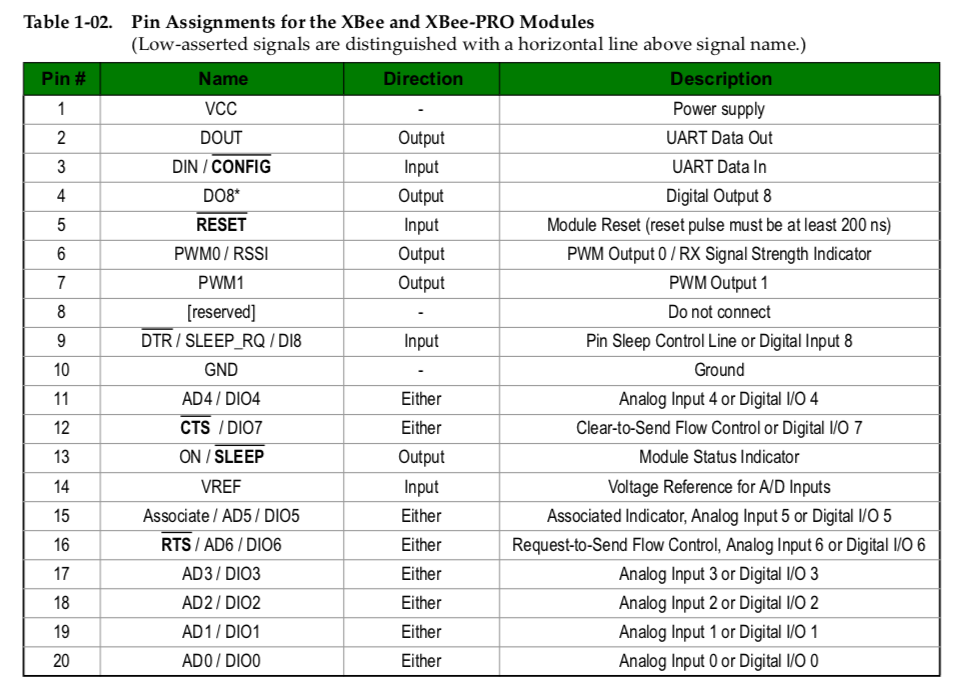
\includegraphics[width=1\textwidth]{figs/img/XBeePinConfig}}
  \caption{XBee Pin Configuration}
  \label{fig:XBeePinConfig}
\end{figure}

\begin{figure}
  \centering
  \boxed{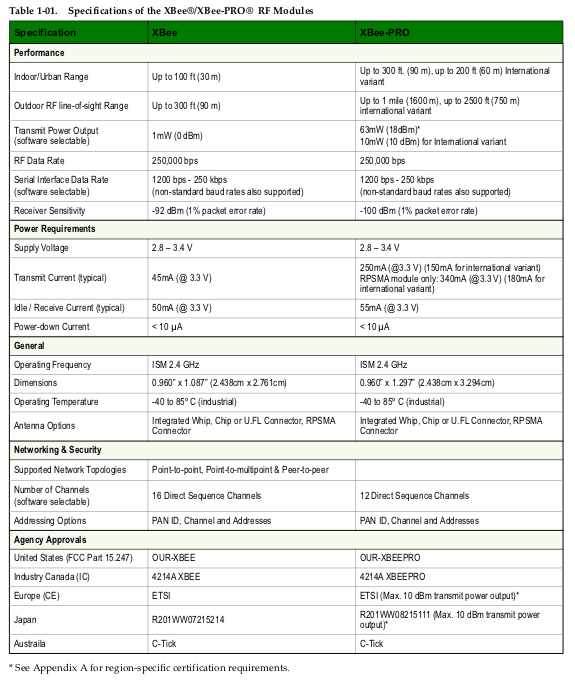
\includegraphics[width=1\textwidth]{figs/img/XBeeData}}
  \caption{XBee Data}
  \label{fig:XBeeData}
\end{figure}

\begin{figure}
  \centering
  \boxed{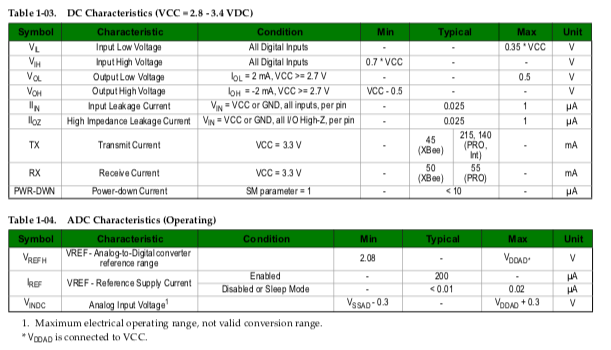
\includegraphics[width=1\textwidth]{figs/img/XbeeElectricData}}
  \caption{XBee Electric Data}
  \label{fig:XBeeElectricData}
\end{figure}

\labday{September 11, 2018}
The group obtained a XBee S2C module and downloaded the software that interacts with them on Reece's laptop. We started to download the same software on the Rpi in attempts for ease of debugging and interfacing in the future. 
Jordan began using the deer library. I started to model the current motor schematic in Simscape for use later when we require more complicated schematics. 
Bob was trying to interface the WeMo switch as well as get BEMOSS to work. He has recognized that the switch that has not been able to work is probably because it is not one of the recognized devices, it is instead a newer version that has changed architecture. Because of the new architecture the code does not recognize what the switch is and BEMOSS will not work. He also updated raspberry pi so emacs could be installed.

\labday{September 13, 2018}
Xbee Set up 16:40: 
we used a USB to XBEE board to configure the XBEE on the XCTU software. 
\newline PAN ID: 1234 (all modules in network must have same PAN ID
\newline DL Destination Address: 415B96BF
\newline NI Node Identifier: RPi
\newline SH: 13A200
\newline SL: 415B96A7
\newline DH:0
\newline DL:FFFF 
\newline modules transmissions received by all modules 
XBee Set Up 16:32
\newline Pan ID: 1234
\newline DL: FFFF
\newline NI Node Identifier: MotorDrive
\newline SH: 0013A200
\newline SL: 415B96BF\\
SL: 41630E56
\newline set up 3
\newline Channel C
\newline PAN ID: 1234
\newline DH=DL=0
\newline MY=16 bit source address =0
\newline SH=13A200
\newline SL: 41630E56 


% set DH=SH and DL=SL on each XBEE to talk to eachother 

\labday{September 14, 2018}
Robert has learned that the current devices we have are not BEMOSS compatible and will double check that the plug controller he is planning on purchasing is compatible. Will send the list of items that need purchased by next week.
\newline
\newline
Reece has started configuring the Xbees, they should be able to communicate with one another but we have not been able to test it yet as we only have one Xbee dock.
\newline
\newline
We will connect the xbee to the raspberry pi and send the signal to another xbee which should be able to control the motor driver.
\newline 
\newline
Dr. Miah will work with Jordan to formulate the problem for the paper. The simscape model will be worked on and simulated. The h-bridge needs to be added to the model and a varying PWM model based on the hardware in the lab. A real-time simulation and result will be modeled.
\newline
Items to purchase:
\begin{itemize}
    \item Plug controller
    \item micro-usb plugs
    \item xbee dock
\end{itemize}

\labday{September 18, 2018}
Jordan has completed the model of the current hardware setup in simscape. 
\begin{figure}
  \centering
  \boxed{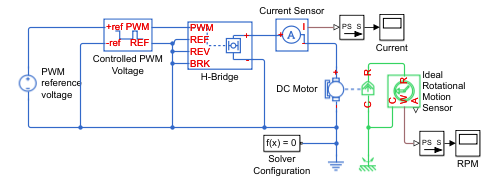
\includegraphics{figs/img/motorModelWithHBridge.png}}
  \caption{Simulink Model of Motor with H Bridge Control}
  \label{fig:motorModelWithHBridge}
\end{figure}
\newline
Bob and Reece have been working on the XBee and getting a better understanding of the zigbee protocol. We are attempting to connect from what will be the transmitting board to the receiving board and just set a pin high. If we are able to do this then we will find out what we will have to do in python to transmit the signal from the transmitting XBee to the receiving XBee so that we won't have to send the packet every time.

\labday{September 20, 2018}
Today Bob and Reece were working to try and get XBee's to communicate with each other. we are trying to use XCTU in order to send a command from the transmitter to the receiver in order to enable a pin high. The current AT command that we are looking at is giving us trouble due to the fact that XCTU does not document what we have to do in order to create a frame. While using the frame generator we are able to create a frame with the correct directory address but we do not know the command to set the pin high. 

\labday{September 21, 2018}
Starting on the high level structure that was agreed upon. Reece should attempt to create the block diagram in IPE. Jordan should assist Reece in creating the high level structure in IPE.
 \newline 
 \newline
 Dr. Miah has shared a document with us that will the the deliverable for Thursday the 27th and Reece will be writing the system architecture. Jordan will be able to assist Reece in writing that.
 \newline
 \newline
 The problem of Deep reinforcement learning must be understood still. We want to apply the technique into BEMOSS to determine the difference between energy consumption with and without deep reinforcement learning. The final outcome of the deliverable should be about 3 pages. Reading other papers should give us a good understanding of what we are going to need to do for this. The Project description should be understandable by many people, not very difficult or specifics. Describe each and every block. Make sure the descriptions are not too specific. 
 \newline
  Robert will be writing the project description. Project description should be at least half a page, read some other papers to get a better understanding of what it should look like.
 \newline
 Jordan and Reece will be working together on Modes of Operation. Modes of Operation, try and have 3 or 4 modes 
 \newline
 \newline
 Jordan should have a complete set up in simscape for what we are doing. In order to do so we still need simscape electrical toolbox. Jordan has it on his laptop so he will be working on the simulink model. Jordan should be a simscape expert and model everything.
 \newline
 \newline
 There is a good resource to look at in order to interface from the WeMo switch to BEMOSS called fauxmo.
 \newline
 \newline
 We should show our interface wireless to the motor. To start out we just need to get the work done and then once that is done we can make it look pretty.
 We need to have the document done by next Tuesday, the 25th. HVAC should be in simscape electrical so interfacing with it should be doable.
 
 
 
 \labday{Monday September 24}
 Reece's XBEE research: 
 Found on https://www.cooking-hacks.com/documentation/tutorials/xbee-arduino-raspberry-pi-tutorial \newline 
 \newline If a module's DH is 0 and its DL is less than 0xFFFF (i.e. 16 bits), data transmitted by that module will be received by any module whose 16-bit address MY parameter equals DL \newline 
\newline If DH is 0 and DL equals 0xFFFF, the module's transmissions will be received by all modules. \newline 
\newline If DH is non-zero or DL is greater than 0xFFFF, the transmission will only be received by the module whose serial number equals the transmitting module's destination address (i.e. whose SH equals the transmitting module's DH and whose SL equals its DL ).
\newline 
\newline Successful Frame transmit to set IO4 on remote xbee high: 
\newline 7E 00 10 17 01 00 13 A2 00 41 63 0E 56 FF FE 02 44 34 05 AE
\newline 
\newline Successful Frame transmit to set IO4 on remote xbee low:
\newline 7E 00 10 17 01 00 13 A2 00 41 63 0E 56 FF FE 02 44 34 04 AF
\newline 
\newline Successful Frame transmit D3 High: 
\newline 7E 00 10 17 01 00 13 A2 00 41 63 0E 56 FF FE 02 44 33 05 AF
\newline Successful Frame Transmit D3 Low: 
\newline 7E 00 10 17 01 00 13 A2 00 41 63 0E 56 FF FE 02 44 33 04 B0
\newline Below is a very useful resource for XBEE 

today in lab, Reece successfully toggled pin 3 and 4 of the remote xbee high and low through the XCTU software and the controller xbee. Note that the address to send frames to can disappear when the controller node is disconnected from power.  
\begin{figure}
  
  \boxed{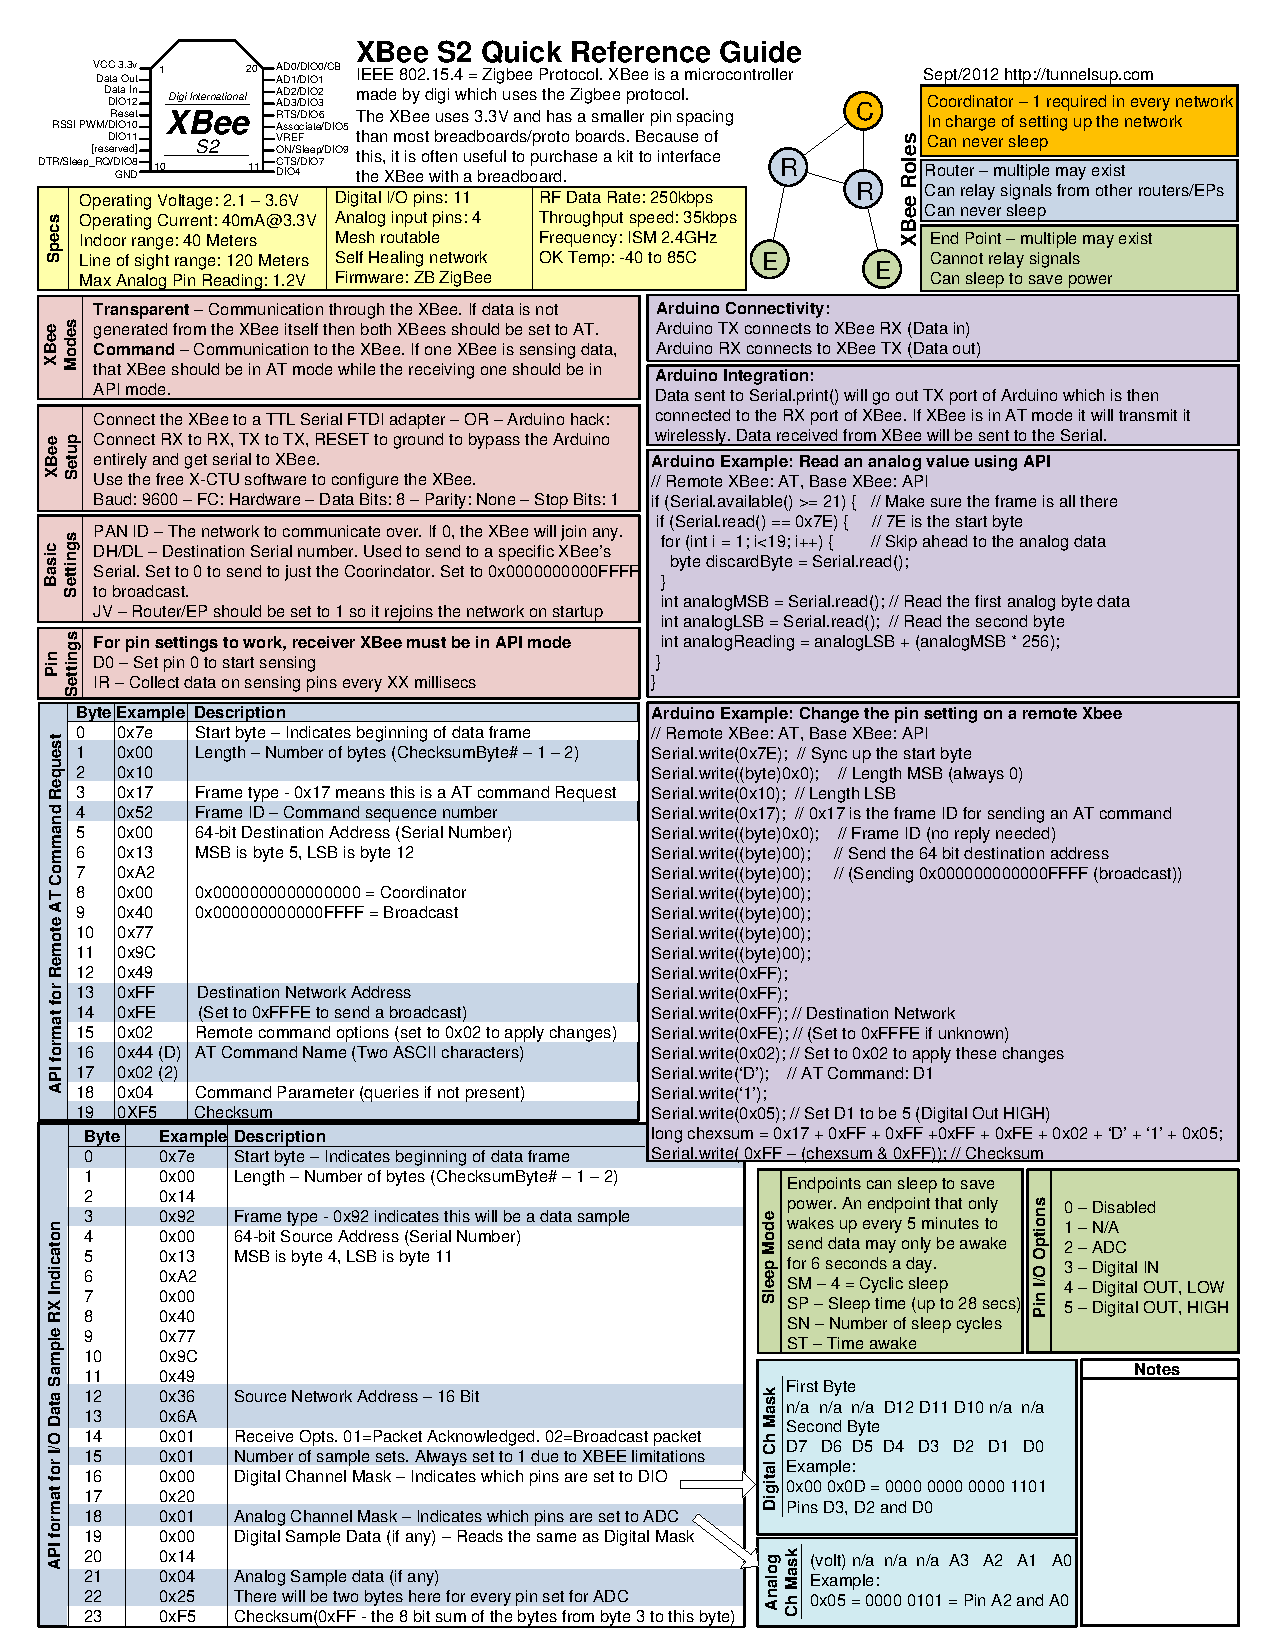
\includegraphics[width=0.5\textwidth]{figs/img/XBee-Quick-Reference-Guide.pdf}}
  \caption{Xbee Quick Reference Guide}
  \label{fig:XBee Quick Reference Guide}
\end{figure}

\labday{Tuesday September 25,2018}
We started work on connecting the base Xbee to the raspberry pi. The pi is supplying 3.3V to the xbee, a ground, and the TX pin on the pi is connected to the DIN pin on the xbee. we are working to serially transmit the hex codes above into the base pi and monitoring the pins on the receiver to see if they toggle. We are working to download the proper libraries and understand the code to use the TX pin/ UART on the pi. 

We completed our rough draft of our project proposal and sent it to Dr. Miah for approval. 

\labday{Thursday September 27,2018}
We worked on polishing up the our project proposal which needed to be turned in today. Following the suggestions by Dr. Miah we were able to make it look much nicer than before the revisions. After finishing working with the project proposal we worked on getting the communication from the raspberry pi to an XBee through serial connection. As of now we are having issues understanding the port that we need to open in order to use the communication to an XBee. 


\labday{Tuesday October 2, 2018}
We successfully controlled the motor through the XBees today. With the base xbee connected to XCTU in our laptops, we remotely toggled pins 3 and 4 of the MD xbee. A jumper on the motor driver needs to connect the ENA pin to the 5v pin on the motor driver board to give a PWM signal of 100 for the motor to turn. The 5v pin is located on the left side of the jumper set directly above the VMS port on the motor drive. The direction of rotation was successfully changed through sending different combinations of the pins. We must be aware to not set both I1 and I2 high at the same time as that would result in a short circuit to ground. At the end of our lab day, the base radio (the xbee connected to XCTU) stopped receiving responses from the MD XBee and the MD Xbee stopped toggling it's pins when commanded to do so.

We updated the raspberry pi and started over using the serial port. We set tty0 as our port. We changed our script setting up the port which now makes the port read as open. In the python script we converted the hex string to a binary string which we are able to send to the xbee. We are not sure if the string will need to be converted to a binary int as the xbees stopped responding at the end.


\labday{October 4, 2018}
Meeting with Dr. Miah: 
Our parts have arrived and will be picked up from Mr. Mattus today. 
Jordan's update: working with transmitting hex values through the pi. Has not completed research on the algorithm or simulating the grid. 
\begin{itemize}
\item Send an email with 2-3 bullet points of exact name of toolboxes needed to do our project
\item research existing algorithms and models to implement 
\item put Jordan's Simulink model in Google drive>simulation
\item model every bit of hardware that we are using in simulink 
    -come in handy for energy savings 
\end{itemize}

Bob's update: has been working on controlling the Xbee with the pi. 
-wants to see functioning control of devices through BEMOSS on Thursday 
-do research on implementation of WeMo switch 

aspirations of writing conference paper regarding our progress and research by semester's end. 
Reece research how to control xbee over rpi. 


With the new USB Xbee explorer, we were not able to discover the old remote xbee, which leads us to think that it has completely failed. We obtained a new xbee and discovered it through XCTU with no problems. Bob 


\labday{October 11, 2018}
Reece set up a new remote xbee to replace the one that failed. Below are the new frames to toggle pin 3 and 4 low and high: 

\vspace{1.0cm}
\noindent
Successful Frame transmit to set IO4 on remote xbee high: 
\newline 7E 00 10 17 01 00 13 A2 00 40 DD E2 88 FF FE 02 44 34 05 2F
\newline 
\newline Successful Frame transmit to set IO4 on remote xbee low:
\newline 7E 00 10 17 01 00 13 A2 00 40 DD E2 88 FF FE 02 44 34 04 30
\newline 
\newline Successful Frame transmit D3 High: 
\newline 7E 00 10 17 01 00 13 A2 00 40 DD E2 88 FF FE 02 44 33 05 30
\newline Successful Frame Transmit D3 Low: 
\newline 7E 00 10 17 01 00 13 A2 00 40 DD E2 88 FF FE 02 44 33 04 31
\newline
\newline Through this, the pins are successfully toggled. The remote pins were reattached to the motor driver and the motor turned as expected. The motor was left running for 5 minutes and was routinely switched directions to test if the remote xbee would fail like the previous one did. No problems came of this. I then proceeded to move the base xbee from my laptop to be controlled by the Pi. There are issues in transmitting the hex values through the Tx Pin on the PI. I hooked up the RX pin on the PI to the Tx pin on the pi to see what the pi was sending the xbee. My conclusion is that the pi is currently sending a string to the xbee instead of the hex values that instruct the xbee what to do. There is a severe lack of documentation on this whole process, so some further exploration is needed here. 

Robert
\newline Today I was attempting to get my virtual machine to connect to the Insight switch but ran into a few problems along the way. The first problem that I encountered was with the bridge network that I was attempting to connect my virtual machine to. My computer is currently denying access from bridging the network that I am connecting on to another network. This is causing problems within my guest machine because I am considered to be connected to a network but I am not able to use the internet on the guest machine. 


Jordan
\newline
I have updated the model of the motor in simscape. I have added a power measurement to track the energy usage for use when we implement an algorithm to reduce power consumption.

\labday{October 12, 2018}

During the meeting today we discussed a few of the issues that we are having with Dr. Miah. 
Deadline for the conference paper that we will be working on is November 19. We have been given the paper template and Jordan is going to write the algorithm. Robert will image a new sd card to have ubuntu 16.04 on it to try and get BEMOSS running on the pi properly. Reece will be working on making the motor look more professional by mounting a few of the things together. Make sure that what is being done is modular so that future students can work on it. 3D printing might be a good option in order to make it look professional. Robert will be working on a new raspberry pi to try and get Ubuntu running on it.




\labday{October 16 2018}
Bob and Reece successfully got a BEMOSS server running on Reece's macbook and connected to its IP adresss. We connected Reece's laptop and the WEMO switch to Reece's iphone hotspot and ECE-Robotics1 at two different points in time and still could not find the switch. Oddly enough, we found a BEMOSS weather sensor on our server when we don't have a BEMOSS weather sensor. 
\newline
Jordan set up a HVAC system in simscape to simulate the power used in a sample HVAC system that will be made more efficient using an already made algorithm and later a neural network algorithm.


\labday{October 18 2018}
Bob and Reece were attempting to get the raspberry pi to transmit data serially to itself currently and in the future try to transmit the data wirelessly to the XBee. Currently we are having an issue with the python code that we are writing. Both of us were attempting to write the AT and API commands within the python code that we are writing. The issue currently is that the libraries that we are trying to use are not being done properly. The first issue is that pip install XBee returns an error. Due to this we cannot use the library and cannot determine of the code that we are writing is working.

\labday{October 23 2018}
Today we decided to switch from communicating directly between two Xbees to running the reciever Xbee to another raspberry pi to allow us to send commands as strings rather than as hex values. This will allow us to more easily control the direction and easily control the pwm. In order to do so we are using the XBee package in python 2. This will allow us to communicate from the raspberry pi to the XBee much easier than if we were to try and do everything from scratch. This had also been a big issue for us due to the fact that our previous raspberry pi wouldn't download the essential xbee package. Trying to do so on a fresh raspberry pi allowed us to install the XBee package and now we are attempting to understand the package and using that.



\labday{October 25 2018} 
Mr Mattus assembbled a mount that attatches on top of our motor that we can use to mount our electronics on top of. The motor and wiring now looks clean and relatively professional. 

\missingfigure{Please add the picture of the assembled motor here.}


I have plans to attatch power ports to the mount to clean up the top and place a 5-3.3v regulator on the bread board to eliminate 2 wires to the board and the need for a second power supply. All-in-all this should take 5 minutes. 

The newly installed xbee package is working and allowing us to further our project. We still have not succesfully sent a command from the pi, so we trouble shot by connecting the TX and Rx of the pi. Below is our error: 
Traceback (most recent call last):

\begin{verbatim}
File "serial_transmit.py", line 23, in <module>
    response = xbee.wait_read_frame()
  File "/home/pi/.local/lib/python2.7/site-packages/xbee/thread/base.py", 
  line 107, in wait_read_frame return self._split_response(frame.data)
  File "/home/pi/.local/lib/python2.7/site-packages/xbee/backend/base.py", 
  line 177, in _split_response data[0], cmd_name)
xbee.backend.base.CommandFrameException: 
"Incoming frame with id \x17 looks like a command frame of type 'remote_at' 
(these should not be received). 
Are you sure your devices are in API mode?    
\end{verbatim}
  


This error shows that we are transmitting (what we believe to be) the proper command, but the xbee seems to not take this command and transmit our command itself.

Jordan updated the paper adding sections on the models for the motor and house. These models have been built in simulink/simscape. Previous when simulated together the model would take over one day to simulate. after separating the models the simulation was able to be run in under one minute. I am currently researching distributed control to be used in the control design in the future. 


\labday{October 26, 2018}
Reece tested the new Wemo insight switch on his home wifi network with no success. Bemoss cannot find the plug when scanning for new devices. The device is able to work with the app on multiple wifi networks. We will schedule a meeting with the Virginia Tech Bemoss faculty to try and resolve this issue. 


\begin{itemize}
    \item Bob needs to send a detail email to Dr. Miah to point out the problem with screen shots. Dr. Miah will use this to schedule a Skype Meeting 
    \item Bob's report: RPi architecture cannot support BEMOSS. 
    \item Kyle's group controled the Xbee serially on a beagle bone black with C code and Rosaria 
    \item Problem statement is due tonight 
    \item Project proposal is due November 6th -include references (atleast 20) 
    \item Dr Miah will share C code with us through our BEMOSS email account that was used in a previous capstone project that used a beaglebone black to serially work with Xbees 
    \item ROSARIA is a robot OS comprised of many libraries. 
    \item the research paper is due sometime in November 
    \item Jordan needs to implement algorithms 
    \item jordan put your reference papers in the notebook 
    \item jordan make graphs accurate 
    \item look at Jacob and Kyle's code at home and figure it out
    \item implement findings in lab 
    \item if Jordan like's the new algorithm, he needs to implement within a week 
    \item Jordan let Dr. Miah know if he doesn't understand any of the symbols 
    \item Jordan demonstrate new algorithm to Dr Miah on Tuesday 
    \item in email, highlight the bright side on what we can do and what we will be able to do and then talk about the dark side of our issues. 
    \item Mr Mattus updated simulink, Bob will check that it works and then we will install it on the robotics lab computers 
\end{itemize}

\labday{October 29, 2018}
Reece put a 3.3v regulator in the circuit to power the XBee. The circuit is now much cleaner and practical as it only uses 1 power supply. The circuit is fully functional and neat now. 

\begin{figure}
  
  \boxed{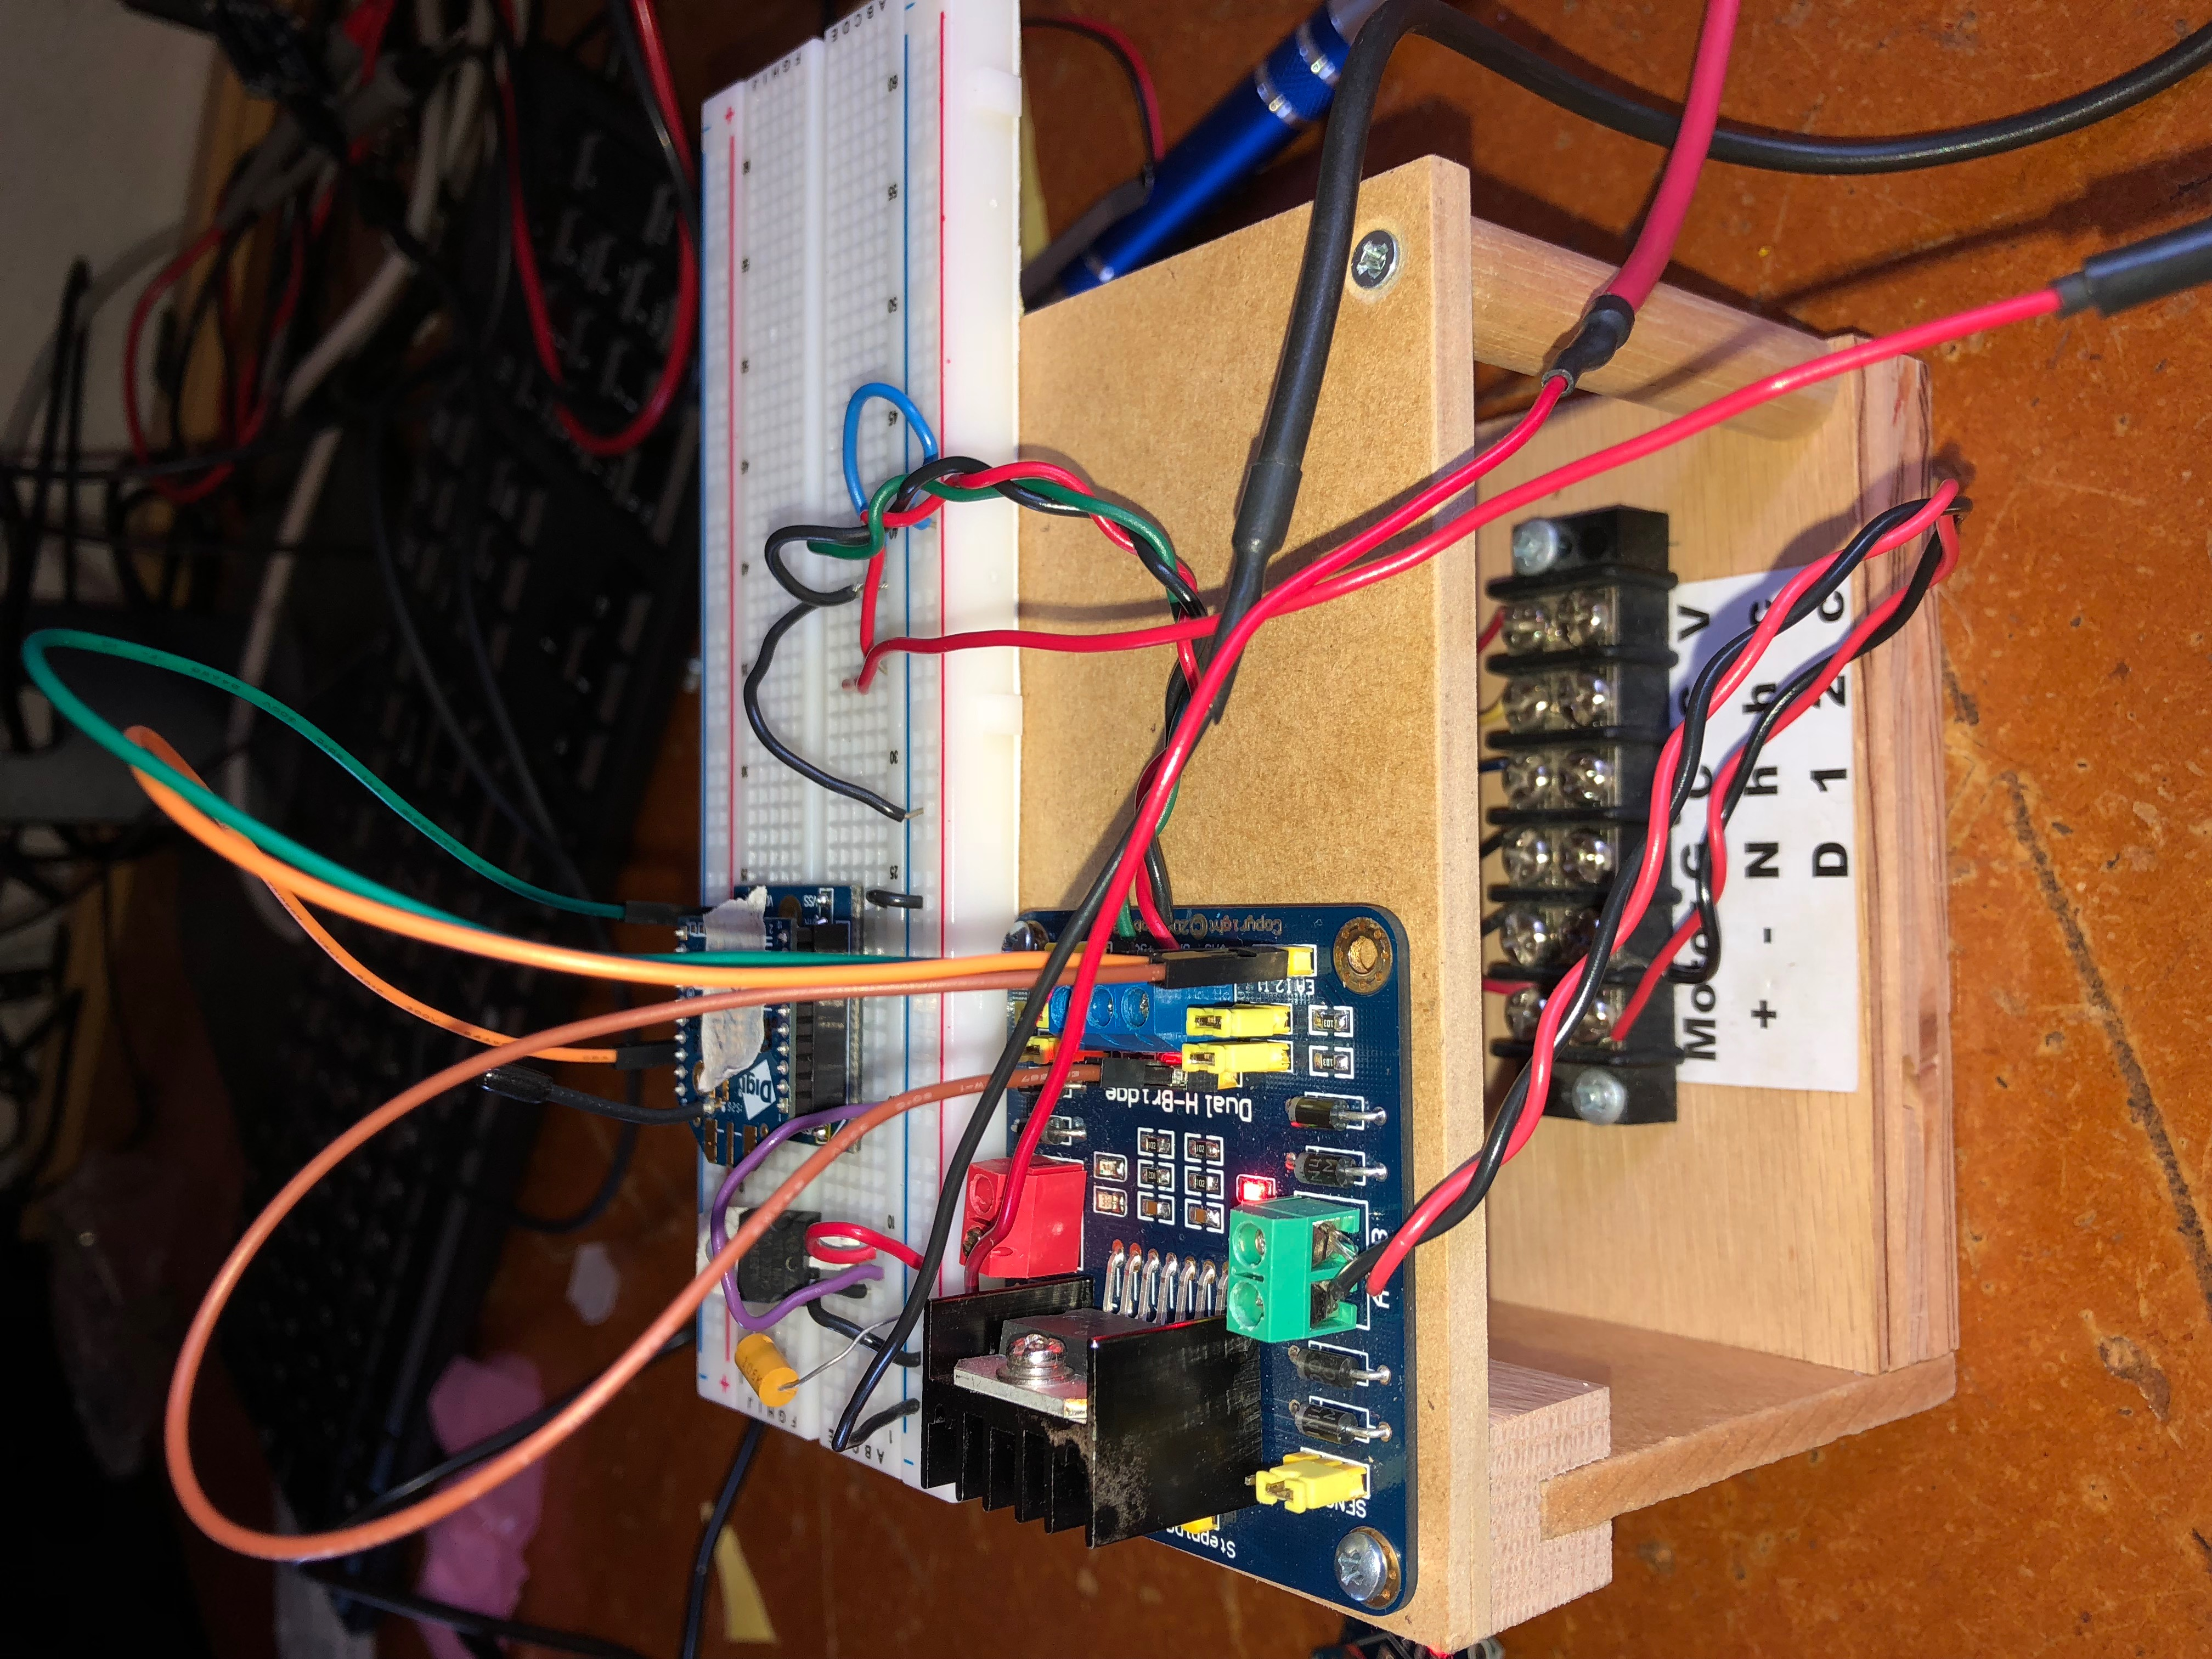
\includegraphics[width=0.5\textwidth]{figs/img/Circuit10_29}}
  \caption{Remote Motor circuit}
  \label{fig:Remote Motor Circuit}
\end{figure}



\labday{October 30, 2018}
Reece found code on the python-xbee library that should be what we need. The python script seems to have issues when it enters the first module to execute AT commands. I think the issue stems from the xbee not being initialized into AT mode properly. 
Bob has been trying different versions of VirtualBox stemming back from 5.21. There are still issues that are occurring with the bridge network that we cannot determine the cause from but we have been able to replicate the issue on Reece's computer as well as on Jordan's computer. This leads me to believe that there is an issue with attempting to create a bridged network while on BUSecure, the WiFi that we most commonly use. 
Jordan worked on modeling the system from the paper from Dr. Miah. Together with Dr. Miah we found another paper that the first paper used to model their HVAC system. From this paper I should be able to develop a state space model that will allow the event based controller.


\labday{October 31,2018}
Reece created a new python script to work with the xbees. This script, titled "XBEETEST.py" is under the same testing scripts folder. It is designed to ping the xbee and obtain he destination address high and low. I used the USB port on the pi to hookup the xbee with time. The code to do this is 

ser=serial.Serial('/dev/ttyUSB0',9600)

This successfully worked, but after turning off the remote xbee it still worked, showing me that it is indeed pinging the coordinator xbee and not the remote xbee. 

I created a new script that compares well with every tutorial related to sending at commands through the Pi. The issue that is stopping me is the destination hex addreses are too large to convert into ASCII values (the error reads 
"UnicodeEncodeError: 'ascii' codec cant encode characters in position: oridnal not in range(128) 

I tried changing the destination address to "FFFF", which broadcasts to every xbee in the area, but the same error prevailed. If this issue can be sorted out, we should be in business. 

\labday{November 1, 2018}
Bob
Today during lab I exhausted all of the options that I believe I had to try and get the bridge network to work. Following up from yesterday I have been experimenting with different network and controls options within Windows 10 itself and I have not been able to make any progress so far. 
Jordan
I continued to work on the model. There have been issues with the understanding of the dynamic system analysis since I have not taken the class yet but I am making strides in order to get it to work.

\labday{Noveber 2, 2018}
We are working with HVAC algorithms currently because BEMOSS does not have any supported algorithms.

in the presentation we must discuss the division of work between us as well as what our main three ideas for our project are which are listed below,
\begin{itemize}
    \item Introduce new BEMOSS device
    \item get BEMOSS to work on a new device like raspberry pi
    \item Develop algorithm for BEMOSS
\end{itemize}
Presentation Deadline: November 13
Proposal Deadline: November 6
Make sure that we do not divert from the 3 objectives.
Paper deadline: November 19
Jordan needs to model one zone and just one zone in simulink in order to determine that the algorithm works. Might want to ask professor Wang about the questions that you have during class.

Bob needs to try a whole new virtual machine on someone's home internet like Jordan so that we can determine if this is an issue with BUSecure. Download an old version of VirtualBox as well as ubuntu 16.04 so that we can know if there is an issue with what software I was using.


\labday{November 6, 2018}
Reece successfully used the raspberry pi to serially transmit to the xbee coordinator and control the remote motor. The python script that controls the xbee is "XBEETEST.py". The script send the commands to toggle the remote pins at different intervals, thus changing the direction of the motor rotation every 2 seconds. A major issue that we resolved is the port that we are talking to. Rpi 3 model A uses AMA0 to communicate with the RX and TX pins. The issue with this is that port on Rpi 3 model B is the bluetooth connection. To use the RX TX pins on the model b, ttyS0 is to be used. 

The code is as follows (can also be seen on the attatched XBEETEST.py file) : 

\begin{mdframed}[backgroundcolor=yellow!5, roundcorner=10pt,outerlinecolor= blue!70!black,outerlinewidth=1.2,frametitle=XBEETEST.py]
\inputminted[linenos=true]{python}{codeFiles/pythonCode/xbeeTest.py}
\end{mdframed}


\labday{November 8, 2018}
Reece 
\newline I did further research and found that Rpis seem to be prevalent in a lot of previous work (at least the figures provided suggest that). See image below from the Department of Energy.
In addition, I started pursuing a closed loop system to allow for accuracy in the actual environments that this motor will be applied in. I debated with bob whether using a bump switch or the built in encoder would be best suited to provide feedback. We concluded that using the encoder on the back of the motor would allow for the greatest flexibility and ability for the future applications. After not being able to find the data sheet for the encoder on the back of the motor, I sent an email to Mr Mattus to see if he knows. Once I find this information out, I will probe the output of the encoder while the motor is running to see what kind of data it spits out. 

I also researched how to send data from our remote xbee to the coordinator xbee. This new settings were put in place and should be ready to test with the encoder. My goal is to have a python script that can send a remote AT command from the coordinator to turn the motor and then receive data from the remote xbee on where the motor position is. Through this, we could locate the position of a door or curtain. The remote xbee should be able to sample and send data on it's own without the help of a single board computer. 


\begin{figure}
  
  \boxed{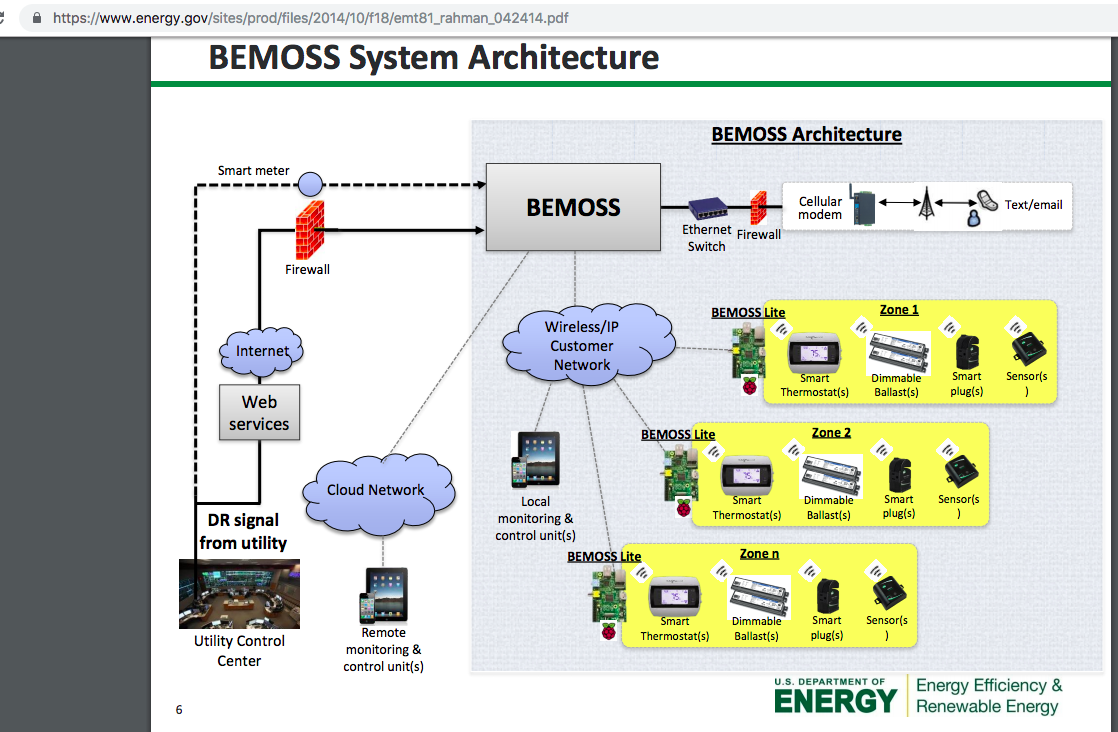
\includegraphics[width=1\textwidth]{figs/img/BemossDOE.png}.png}
  \caption{Bemoss DOE Architecture}
  \label{fig:XBee Quick Reference Guide}
\end{figure}

Bob
I have been researching a dual boot for my computer to try and make the network settings easier for BEMOSS. If I set up my computer for a dual boot then there will not be a need for a forced IP when doing a bridge network. This might allow BEMOSS to discover the supported devices and be a good fix.

Jordan
I have been working on the system model from the research paper. Currently the problem is that T\textsuperscript{e} is defined in the paper as a N+1 vector while the rest of the variables in the equation are defined as scalars. This is not allowing me to move on as the matrix sizes do not align. I will continue looking at the equations from the paper to figure out where this confusion is coming from.

\labday{November 9, 2018}
The presentation will be on Thursday, November 29, at 10:15-10:40. Practice for presentation will begin at least one week before the presentation. The presentation will be recorded and sent to the industry advising board. Presentation will be around 20 minutes with a 5 minute question answer. 
\begin{itemize}
    \item Bob needs to talk to Mr. Mattus to get a new laptop with administrative privileges and install Ubuntu 16.04. After I get the laptop I will send an email to Ashraf to set up another meeting to get BEMOSS running from scratch. 
    \item Tuesday, November 20 from 8:00 to 8:30 we will be practicing our presentation.
    \item Jordan is going to meet with professor Miah at 12:45 until around 1:50 and then from 4:00 to 5:00 to try and work through the paper. 
    \item Reece needs to get a boost converter as well as a converter from 5 to 3.3V to get the encoder to work as intended
\end{itemize}

\labday{November 11, 2018}
\experiment{HVAC Modeling}

\begin{multline*}
    \label{eq:HVAC-Modeling}
    \frac{\mathrm{d}\mathbf{T}^e}{\mathrm{dt}} = 
    \begin{bmatrix}
    \dot{T}_1^e\\
    \dot{T}_2^e    
    \end{bmatrix}
    = 
    \begin{bmatrix}
    -\frac{u_{cc}A_{cc}}{M_{cc}C_v} & \frac{Q_w\rho_w C_{\rho_w}}{M_{cc}C_v}\\
    0 &  -\frac{Q_w\rho_wC_{pw}+U_tA_t}{V_t\rho_wC_{pw}}
    \end{bmatrix}
    \begin{bmatrix}
    T_1^e\\
    T_2^e
    \end{bmatrix}
    +
    \begin{bmatrix}
    \frac{U_{cc}A_{cc}}{M_{cc}C_v}T_{amb} - \frac{Q_w\rho_wC_{pw}}{M_{cc}C_v}T_{wo} \\
    \frac{U_tA_t}{V_t\rho_wC_{pw}}T_{amb} + \frac{Q_w\rho_wC_{pw}}{V_t\rho_wC_{pw}}T_{wo}
    \end{bmatrix}
    +\\
    \begin{bmatrix}
    0 \\
    \frac{15000}{V_t\rho_wC_{pw}}
    \end{bmatrix}
    \chi
    +
    \begin{bmatrix}
    (\frac{\rho_aC_{pa}}{M_{cc}C_v}Q_{a1}-\frac{U_{cc}A_{cc}}{M_{cc}C_v})\\
    0
    \end{bmatrix}    
\end{multline*}

\labday{November 13, 2018}
Reece ran through the data sheets of the encoder mounted on the back of our pittman motor. The sheets can be found on the department computers under Mis/datasheets/pitman Motor? HEDS. These sheets say that power supply to the encoder must be between 4.5-5.5v. I tested the encoder with success and found that one channel will lead the other depending on the direction of rotation. I am also in the process of ordering a 5v-3.3v logic converter to transmit the output of the encoder over the xbees. 
Bob
I was looking over some of the code within BEMOSS to try and get a better understanding of how to interface a device once we have it working. A lot of the API's a very different from each other because each device runs off of a different protocol. We are going to be trying to reference one of the devices that will be using zigbee protocol since that is what we are planning to use for our project.


%\begin{center}
%\centering
    \begin{tikzpicture}
      \tikzstyle{every node} = [font=\tiny]
      \tikzstyle{block} = [draw, rectangle, fill=blue!20, rounded corners, minimum height=1.0 cm, minimum width=2.2 cm]
      \tikzstyle{sum} = [draw, circle, fill=gray];
      \tikzstyle{pinstyle} = [pin edge={to-,thin,black}]
      \node[sum](sum){$\sum$};
      \node[block, text width=2 cm, text centered, right of = sum, node distance=2 cm](controller){Controller: $\rho_i(t) = K_Pe(t) + K_I\int_0^te(t)\mathrm{dt}$};
      \node[block,text width= 2 cm, text centered, right of=controller, node distance=3.5 cm](BLDCMotor){Three-phase interver + BLDC motor};
      \node[block,text width= 2 cm, text centered, below of=BLDCMotor, node distance=1.5 cm](HallSensor){Current sensor, Hall sensor};
      \node[block,text width= 2 cm, text centered, below of=controller, node distance=1.5 cm](signalConditioning){Signal conditioning unit};
      % Connections
      \draw[<-]
      (sum) --++(-\myGrid,0) node[midway, above]{$\omega_r$};
      \draw[->] 
      (sum)--node[midway,above]{$e(t)$}(controller.west);
      \draw[->]
      (controller.east)--node[midway,above]{$\rho_i$}(BLDCMotor.west);
      \draw[->]
      (BLDCMotor.east)-- node[midway,above]{Position, $\theta(t)$}($(BLDCMotor.east)+(1.5*\myGrid,0)$);
      \draw[->]
      ($(BLDCMotor.east)+(0.5*\myGrid,0)$) |- (HallSensor.east);
      \draw[->]
      (HallSensor.west) --node[midway,above]{Hall A, B, C}(signalConditioning.east);
      \draw[->]
      (signalConditioning.west) -| node[midway,below]{$\omega(t)$}(sum.south);
      \draw
      ($(sum.south east)+(0.01*\myGrid,-0.15*\myGrid)$)node{--};
      \draw
      ($(sum.south east)+(-0.6*\myGrid,0*\myGrid)$)node{+};
      % Layers
      \begin{pgfonlayer}{background}
        \filldraw[line width=10mm,join=round,gray!10]
        ($(signalConditioning.south west) + (-0.8*\myGrid,0.2*\myGrid)$) rectangle (BLDCMotor.north east);
      \end{pgfonlayer}
      \draw
      ($(controller.north west) + (0,0.3*\myGrid)$)node{Motor controller unit};
    \end{tikzpicture}    
\labday{November 16, 2018}
Bob will come to Jordan's house on Saturday and re install BEMOSS on the lapotop he recieved from Mattus.  

Jordan needs to find Qa1 and chi as a function of T1e, T2e, and Tze

Conference paper for Florida due by 11:55 on November 19. Rough draft of presentation needs to be sent to Dr. Miah by Sunday as well.

Reece has been looking at parts to order. He has put together a list and sent the list to Mr. Mattus. Mattus will check with the current parts the department has and order the others. Reece will put his current work in paper format for Purposed Supported BEMOSS Device, which will be part of the proposal, paper, and presentation.

Jordan will send an email to Lu and cc to Suruz explaining the situation with MATLAB asking for an extension. If Jordan cannot get his MATLAB to work tonight he will email Dr. Miah tonight or tomorrow morning to work in the lab.

Reece will work on creating a feedback system. From the system we will develop a mathematical model in statespace and from their define a cost function to minimize the energy cost.

\labday{November 27, 2018}
Today we went over the presentation that we will have on November 29 at 10:15 am. Robert and Reece have created videos highlighting the current results of our project. 

Reece installed the new buck/boost converter we purchased. This allows us to run the motor off of one power supply rather than two.


\labday{November 30, 2018}
We will not have a meeting next week due to finals. Before the end of the semester we will have one more meeting to set up the plan for next semester. We will arrange a time that works for us after all of our finals and Reece will email Dr. Miah. 

The website needs to be set up and the deliverable need to be on the site by the end of the semester. Use the website from Kyle and Jacob from 2017 as a reference.

\labday{December 11, 2018}
We need to add a more to the website, does not need to be fancy yet.
\begin{itemize}
    \item Problem description
    \item Simulation Results
    \item Pictures of hardware setup
    \item Interfacing with BEMOSS
\end{itemize}

Fall 2018 Deliverables (Name of Doc [link to pdf])
\begin{itemize}
    \item system functional requirements
    \item subsystem level functional requirements
    \item Project proposal
    \item Project presentation
    \item Lab notebook
\end{itemize}
Spring 2019 Deliverables: Just put in progress.
Send an email to Dr. Miah once the website is completed, it needs to be completed for grades.

Over break we should do some research on how to implement our work from this semester, to finalize our work for the project.

Reece and Bob need to email Dr. Ahn to get added to ECE 499.
We need to enjoy our break, we're gonna need it.
Come back fresh for more challenges!

\labday{January 23, 2019}
We will have our weekly meetings this semester on Tuesday from 11:45am-12:30pm.
Weekly lab days on Tuesday from 9am-1pm, Thursdays from 9am-5pm.
Over break Reece did some work on a similar motor encoder.

Start lab work on January 24, Bob will start work on finding the motor and connecting the motor driver to BEMOSS.

Finding the Raspberry Pi on BEMOSS would be a significant step forward. 
Reece and Bob make design on how to interface the Pi with BEMOSS before lab (what APIs talk to what things). 

Jordan needs to update the lab notebook on what he updated in the proposal report. Jordan meets with Dr. Miah on Friday to work on the algorithm 

Website needs to be properly done now. Make it professionally done with proper documentations. 

\labday{January 24, 2019}
As the hardware portion of the project is in a comfortable spot, the team has shifted our focus onto the software aspect. Our initial steps have been to dissect and understand the existing code that allows BEMOSS to connect to the WeMo plug. The code is complicated and involves numerous subroutines. An initial thought that we developed is to throw a subroutine in the existing WeMO API that allows us to send commands to the Raspberry Pi. Bob beleives he has a general idea of what to send, but is unsure on the actual execution. Bob has contacted Ashraf to see if he has insight that could help us get a footing on the next leg of the project. Further steps will include further analyzing the code. Bob and Reece will check with Mr. Mattus if we would be able to take the linux laptop to the library which offers bigger screens to analyze the code on. 

\labday{January 29, 2019}
Ashraf has sent a reply and Bob will send a follow up email to continue his work. Bob has been looking at the current BEMOSS API by looking at the WeMo switch BEMOSS API and API architecture. Bob will contact Ashraf to schedule a meeting to discuss converting the python code we have developed to a API for BEMOSS. We will go through the BEMOSS python code during a future meeting. In the email contacting Ashraf Bob will explaining the current situation of the project (what we are running, small bit how, show the working device). In the email we will send a video demonstrating the device and asking questions about how to connect to BEMOSS. In the video we need to give a very clear description that can be understood to a general audience, describing the current motor setup.
\newline
Dr. Miah will provide the simulink model he has developed with our group. Dr. Miah will explain the simulink model to Jordan and together they will implement the HVAC system into the model. From the model Jordan will use the LQR MATLAB commands to create a LQR controller and connect the controller to the simulink model. Using the LQR I will develop a machine learning control using either the algorithim in the Reppa paper or through a simple gradient descent method.

\labday{January 31, 2019}
Today Bob was doing research on the different types of architecture that different supported devices within BEMOSS use. One of the parts that was researched was the Philips hue bridge which has some technical details here https://www2.meethue.com/en-us/p/hue-bridge/046677458478
As shown on the website, the Philips hue bridge uses zigbee technology as well as 2400-2483.5MHz frequency band which is the same as that of normal Wi-Fi. This leads me to believe that the bridge is using a network card to connect to the internet and once connected, BEMOSS sends data to the bridge. This is also what happens with the WeMo smart plug stated by the website
https://www.belkin.com/us/p/P-F7C063/

\labday{February 1, 2019}
\begin{itemize}
    \item Make another video to send to Dr. Khan and Ashraf.
    \item Meeting with Dr. Khan and Ashraf
    \item 
\end{itemize}

\labday{February 5,2019}
Reece- I stripped the code off of my personal project that I'm using to interface with Amazon's Alexa. Sinric, the software and program that I use, provides code that can be edited in the Arduino IDE to be utilized on single board computers like the Node MCU. There is also code that can be implemented on a RPI. The beauty of this code is that it is very cleanly laid out in the IDE and allows you to add your own functionality in neat loops. While this effortlessly pairs with Amazon's Alexa, further expanding upon it with BEMOSS in mind shouldn't be an impossibility. I am posting this here because this is still the cleanest set of code that I have seen in my research to utilize in order to understand the workings of an API. 

**Sinric code in Code Files>Sinric In Arduino/ BareSinricCode***
\begin{verbatim}
    /*
 Version 0.1 - March 17 2018
*/ 

#include <Arduino.h>
#include <ESP8266WiFi.h>
#include <ESP8266WiFiMulti.h>
#include <WebSocketsClient.h> //  https://github.com/kakopappa/sinric/wiki/How-to-add-dependency-libraries
#include <ArduinoJson.h> // https://github.com/kakopappa/sinric/wiki/How-to-add-dependency-libraries
#include <StreamString.h>

#ifdef __AVR__
  #include <avr/power.h>
#endif

#define PIN 5


ESP8266WiFiMulti WiFiMulti;
WebSocketsClient webSocket;
WiFiClient client;

#define MyApiKey "fffffff" // TODO: Change to your sinric API Key. Your API Key is displayed on sinric.com dashboard
#define MySSID "yyyy" // TODO: Change to your Wifi network SSID
#define MyWifiPassword "xxxxx" // TODO: Change to your Wifi network password

#define HEARTBEAT_INTERVAL 300000 // 5 Minutes 

uint64_t heartbeatTimestamp = 0;
bool isConnected = false;

 
void turnOn(String deviceId) {
  if (deviceId == "5babbd609da69d4076487256") // Motor Right 
  {  
    
  } 
  else if (deviceId == "5babbde29da69d4076487257") // Rainbow ON
  { 
    //Serial.print("Turn on device id: ");
    
  }
  else {
    Serial.print("Turn on for unknown device id: ");
   
  }     
}

void turnOff(String deviceId) {
   if (deviceId == "5babbd609da69d4076487256") // Night Light OFF
   {  
     //Serial.print("Turn off Device ID: ");
     Serial.println("nightlightoff");
   }
   else if (deviceId == "5babbde29da69d4076487257") // Rainbow OFF
   { 
     //Serial.print("Turn off Device ID: ");
     Serial.println("rainbowoff");
   
  }
  else {
     Serial.print("Turn off for unknown device id: ");
     Serial.println(deviceId);    
  }
}

void webSocketEvent(WStype_t type, uint8_t * payload, size_t length) {
  switch(type) {
    case WStype_DISCONNECTED:
      isConnected = false;    
      Serial.printf("[WSc] Webservice disconnected from sinric.com!\n");
      break;
    case WStype_CONNECTED: {
      isConnected = true;
      Serial.printf("[WSc] Service connected to sinric.com at url: %s\n", payload);
      Serial.printf("Waiting for commands from sinric.com ...\n");        
      }
      break;
    case WStype_TEXT: {
        Serial.printf("[WSc] get text: %s\n", payload);
        // Example payloads

        // For Switch  types
        // {"deviceId":"xxx","action":"action.devices.commands.OnOff","value":{"on":true}} // https://developers.google.com/actions/smarthome/traits/onoff
        // {"deviceId":"xxx","action":"action.devices.commands.OnOff","value":{"on":false}}

        DynamicJsonBuffer jsonBuffer;
        JsonObject& json = jsonBuffer.parseObject((char*)payload); 
        String deviceId = json ["deviceId"];     
        String action = json ["action"];
        
        if(action == "action.devices.commands.OnOff") { // Switch 
            String value = json ["value"]["on"];
            Serial.println(value); 
            
            if(value == "true") {
                turnOn(deviceId);
            } else {
                turnOff(deviceId);
            }
        }
        else if (action == "test") {
            Serial.println("[WSc] received test command from sinric.com");
        }
      }
      break;
    case WStype_BIN:
      Serial.printf("[WSc] get binary length: %u\n", length);
      break;
  }
}




void setup() {
  Serial.begin(115200);
//  ets_intr_lock(15); // all intruptt off
//ets_wdt_disable();
  WiFiMulti.addAP(MySSID, MyWifiPassword);
  Serial.println();
  Serial.print("Connecting to Wifi: ");
  Serial.println(MySSID);  

  // Waiting for Wifi connect
  while(WiFiMulti.run() != WL_CONNECTED) {
    delay(500);
    Serial.print(".");
  }
  if(WiFiMulti.run() == WL_CONNECTED) {
    Serial.println("");
    Serial.print("WiFi connected. ");
    Serial.print("IP address: ");
    Serial.println(WiFi.localIP());
    
      strip.begin();
  strip.show(); // Initialize all pixels to 'off'
  }

  // server address, port and URL
  webSocket.begin("iot.sinric.com", 80, "/"); //"iot.sinric.com", 80

  // event handler
  webSocket.onEvent(webSocketEvent);
  webSocket.setAuthorization("apikey", MyApiKey);
  
  // try again every 5000ms if connection has failed
  webSocket.setReconnectInterval(5000);   // If you see 'class WebSocketsClient' has no member named 'setReconnectInterval' error update arduinoWebSockets
}

void loop() {
  webSocket.loop();
  
  if(isConnected) {
      uint64_t now = millis();
      
      // Send heartbeat in order to avoid disconnections during ISP resetting IPs over night. Thanks @MacSass
      if((now - heartbeatTimestamp) > HEARTBEAT_INTERVAL) {
          heartbeatTimestamp = now;
          webSocket.sendTXT("H");          


  
      }
  } 
}  
\end{verbatim}
/*
 Version 0.1 - March 17 2018
*/ 

----MEETING-------------
\begin{itemize}
    \item Write a piece of python code (possibly in a separate compiler like spyder), are you able to find the physical MAC address of a new device?
    \item Find MAC address or IP address. 
    \item then next step is how to talk to them
    \item then get this code into an API 
    \item The meeting with Ashraf will try to take place on Wednesday Feb 6 and 12 central time. We are waiting for a response from Ashraf to confirm if this time works for him
\end{itemize} 

Continue Lab------
Bob and Reece wrote a quick python scrip on the Pi that allows us to find and print it's own IP address. From here, we plan that we should ping every IP address in the network and compare the first 6 hex values of the MAC addresses that are returned to determine which address is associated with our Raspberry Pi. This would allow us to distinguish which address are Pis. MAC address works for wired raspberry pi's: They all start b8:27:eb

After connecting both the Pi and the BEMOSS laptop to ECE Robotics 1, he was able to ping from the BEMOSS laptop and find the IP of the PI. 

Using python, I am able to get the MAC address and the IP address of the machine that I am working on. It will be difficult to try and discover a new machine without having access to the router since the router is crucial to discovering who is on the network.

Jordan started using another paper to simulate the HVAC system. \cite{Serrano1999} is a more concise and better explains the process to develop the model. The control inputs for the system are the  pumping  rate  of  cold  water  from  the  chiller  to  the  heat exchanger and the circulating air flow rate using the variable speed fan. 
% \begin{verbatim}

% \end{verbatim}
\labday{February 6,2019}
Meeting with Ashraf 

How to integrate the motor we built in the lab with bemoss 


DeviceAPI$>$BaseAPI\_WeMO
3 distinct functions when integrating
1-discovering the device
    -local devices connected to the same wifi network as bemoss is running on
    -send in and discover the MAC address
    -IP too
    -there is a ``discover function''
    -"discovered\_devices" returns MAC and IP
    -return device data for socket returns status (device data status and device data power) 
    -our device needs to return status and speed 
    -
2-Getting Data from device and Sending data to device 
    -Might have to talk to another professor because BEMOSS was not build to control a motor
        -it was meant to control lights and their brightness and HVAC 
        -get data from Fast function 
        -WEMO API
        -3 means its a plug load
        -HTML Temmmplate plugload/plugload.html takes in only specific commands 
        -USing a lighting API would be ideal as it has multiple commands it can send (on and off and brightness) 
        
-Write a python code than can discovered MAc ID and status and send commands (good starting point) 
-then translate into weisbuilding (couldn't make out what he said) 
-this is general format of a software based platform 
-write python code 
-

\labday{February 7, 2019}
Jordan found the state space model, will update after work with values for A,B,C matrices and talk about LQR control to be developed.
Bob will be looking into scapy to find the Pi IP adress.
I was attempting to write code that would discover all of the IP addresses that are on a certain network. As of right now, scapy seems like a great library that is included within python to try and do so. I have ran into a few issues that I am not sure how to resolve yet but I believe there is some issue with administration privileges to access all of the devices on a network. This will be looked into on the weekend and hopefully resolved so work can continue

\labday{February 8, 2019}
Since Jordan has obtained his work schedule he is no longer able to attend the regular meetings. We are working to find a new time slot. We have decided on \textbf{Thursdays 3-4pm}. 
\newline
Jordan will create a simulink model based on \cite{Serrano1999} and present the model during the meeting on Thursday.
\labday{February 12, 2019}
Bob did more research on scapy and discovered that this will be able to assist us in verifying what devices are connected on a network. Reece has been working on this as well and is looking into what functions within are usable and how implementing them will impact how the motor works. Jordan worked on the lqr control for the hvac system.

\labday{February 14,2019}
Jordan was able to thoroughly understand and implement about half of the \cite{Serrano1999} paper. The variables and matrices that are presented after this point have little explanation to them. The \cite{Kang2014} paper may present a solution to this as it uses the same variables (with slight variations) as the \cite{Serrano199} paper and provides different explanations. 

Reece has been researching how to implement things in the Pi's end. While Bob works to discover our Pi and send commands to it through the internet, I am researching how to receive and process those commands from the Pi. Most of the top results in my research involve command line such as: 
\begin{verbatim}
    

Now open the file /etc/network/interfaces in nano editor. We need to edit it, open it with root permissions. Use below command.

sudo nano /etc/network/interfaces
 - Add below lines in the file.

auto wlan0
iface wlan0 inet dhcp
wpa-ssid "WIFI NETWORK NAME HERE"
wpa-psk "WIFI NETWORK PASSWORD HERE"
- Update the localization settings to set the WIFI country. Open the file /etc/wpa_supplicant/wpa_supplicant.conf and make below entries in it.

ctrl_interface=DIR=/var/run/wpa_supplicant GROUP=netdev
update_config=1
country=YOUR COUNTRY CODE HERE 
\end{verbatim}
Some issues that might arise with the pi receiving commands is the scanning of commands being sent might not be picked up. In order to make sure this does not happen, Reece will be researching the implementation of the commands on the pi.
---------------------------------------------------------
Some important Python code to connect to Wifi: 
\begin{verbatim}
    import os, sys

print "[+] Enter this some Option"
print " 1. Active Wifi (up)\n 2. Down Wifi (down)\n 3. Exit"
inp_up_down = raw_input("[+] Enter choice number: ")
if inp_up_down == '1':
    os.system("ifconfig wlan0 up")
    print " Are you want connect to wifi?"
    print " 1. Yes, Conncet\n 2. No, Exit"
    inp_connect = raw_input("[+] Enter your choice: ")
    if inp_connect == '1':
        os.system("iwlist wlan0 scan | grep ESSID")
        masuk = raw_input("Enter name of wifi (ex: @wifi.id): ")
        os.system("iwconfig wlan0 essid "+masuk)
        os.system("dhclient wlan0")
    elif inp_connect == '2':
    print "Thankyou.."
        sys.exit()
elif inp_up_down == '2':
    os.system("ifconfig wlan0 down")
elif inp_up_down == '3':
    sys.exit()
else:
    print "Sorry, Wrong Input!!"

\end{verbatim}
-------------------------------------------
An additional WiFi Python Script found on Github. Allows us to find any wifi network

\begin{verbatim}
    

import wifi


def Search():
    wifilist = []

    cells = wifi.Cell.all('wlan0')

    for cell in cells:
        wifilist.append(cell)

    return wifilist


def FindFromSearchList(ssid):
    wifilist = Search()

    for cell in wifilist:
        if cell.ssid == ssid:
            return cell

    return False


def FindFromSavedList(ssid):
    cell = wifi.Scheme.find('wlan0', ssid)

    if cell:
        return cell

    return False


def Connect(ssid, password=None):
    cell = FindFromSearchList(ssid)

    if cell:
        savedcell = FindFromSavedList(cell.ssid)

        # Already Saved from Setting
        if savedcell:
            savedcell.activate()
            return cell

        # First time to conenct
        else:
            if cell.encrypted:
                if password:
                    scheme = Add(cell, password)

                    try:
                        scheme.activate()

                    # Wrong Password
                    except wifi.exceptions.ConnectionError:
                        Delete(ssid)
                        return False

                    return cell
                else:
                    return False
            else:
                scheme = Add(cell)

                try:
                    scheme.activate()
                except wifi.exceptions.ConnectionError:
                    Delete(ssid)
                    return False

                return cell
    
    return False


def Add(cell, password=None):
    if not cell:
        return False

    scheme = wifi.Scheme.for_cell('wlan0', cell.ssid, cell, password)
    scheme.save()
    return scheme


def Delete(ssid):
    if not ssid:
        return False

    cell = FindFromSavedList(ssid)

    if cell:
        cell.delete()
        return True

    return False


if __name__ == '__main__':
    # Search WiFi and return WiFi list
    print Search()

    # Connect WiFi with password & without password
    print Connect('OpenWiFi')
    print Connect('ClosedWiFi', 'password')

    # Delete WiFi from auto connect list
    print Delete('DeleteWiFi')
    
    \end{verbatim}
    --------------------------
    The base Python WiFi Capabilities url: https://pypi.org/project/python-wifi
    "Python WiFi is a Python module that provides read and write access to a wireless network card’s capabilities using the Linux Wireless Extensions."
    -Alot of these scripts have the ability to automatically connect to a wifi upon startup. This may be an attractive feature for a mass rollout of BEMOSS in a new building. 
    ---------------------
    Meeting with Dr Miah 
    see which bits of python code works to find the wifi networks 
        -could use on Pi or laptop 
        -early april project showing in RenCo 
        -need to get router
        
        
        
\labday{February 19}
Reece's scratch pad of thoughts throughout his research:
-We should pursue an approach to have a script automatically connect to the wifi (as seen in the Sinric code I posted) 
-We should pursue research in SSH
-Do IP addresses of a device change each time they reconnect to a router? 
    -possibly need to change this setting in the router if we need the IP address 
-We need to look further into the light control API of BEMOSS
-We should download PUTTY (if we haven't already) on the laptop. we then input the IP address in the settings 
-See this tutorial for PUTTY and remote control of RPI: https://www.youtube.com/watch?v=rLYhzABso30
-This tutorial seems to not be very flexible in it's setup, but we might be able to sacrifice elegance in our first setup to get it to work 
-NOTE this tutorial allows us to execute python code on our raspberry pi by navigating the terminal from the laptop! This will allow us to execute the script that rotates the motor over the internet. From here we could write different python scripts that solely rotate the shaft in one direction and call them individually through command line and PUTTY. 

\labday{February 22,2019}
Reece and Bob
The Raspberry Pi IP address is 192.168.1.41/24
Putty has been successfully installed on the Laptop, but a "Fatal error" occurs stating that the connection has been refused. This same "Connection Refused" message appears on my (Reece's) macbook version of putty (New Remote Connection) in the terminal utilities when connecting to my personal Pi on my home wifi network. Is this the result of a setting default in Rpi? 


\labday{February 26.2019}
Reece-it seems as of 2016, Raspbian defaults to a disabled ssh. In command line on the Pi, ssh is enabled by typing 
sudo systemctl enable ssh
sudo systemctl start ssh

From here, type the IP (as recorded on February 22 labday, and also found by typing sudo ifconfig in Pi's terminal >wlan0>inet addr) into putty. 

The first time connecting to the Pi over ssh produces a warning box-click accept and proceed. The terminal will prompt to enter the Pi's User ID and Password. 

Upon help from Dr Miah, typing ssh pi@192.168.1.41 into the terminal of the laptop has the same effect as using putty. This also allows for more automation applications.


Bob- After doing researching, I am able to determine every MAC address and IP address that is listed on a certain network using nmap. As of right now this is a bit of an issue since I am doing so using bash instead of python. I have posted the results from the script which shows everything on ECE-Robotics1 network in \begin{verbatim}
    ALL_MACS.TXT
\end{verbatim}
there is a library for python that is used to implement the nmap features of command line into python and so I am trying to get this to work.

Reece and Bob at 5pm session----
We have 4 goals in the next step of our project
\begin{itemize}
    \item Find IP's and Mac addresses on network using python script
    \item Distinguish which relate to a raspberry pi (if possible) 
    \item connect to the Pi's over the internet
    \item Send commands (our test will be to run the motor by using script XBEETEST.py)
\end{itemize}

We successfully used the command line on the laptop to ssh into the raspberry pi over ECE-Robotics-1. The Username and password have been reset back to their defaults (User: pi, psswd: raspberry). We ran XBEETEST.py from the laptop and the script was executed and the motor rotated just as before. Next step is to 

Looking through the documentation for raspberry pi's, the MAC addresses for them are guaranteed to start with B8-27-EB, B8:27:EB, or B827.EB. In our case the MAC address is B8:27:EB:BF:BA:DE.

The IP addr of the PI being 192.168.1.41 does not change each time the Pi starts back up or reconnects to ECE Robotics 1

Bob has a working bash script to scan the network and return all IP and MAc addr. With such a well functioning script, we are contemplating calling this bash script from inside our python scripts to complete the scan. As a proof of concept, we are writing a script to automate the connection, password exchange, directory navigation, and script execution to turn our motor. 
\begin{verbatim}
    #!/bin/bash

#mapfile -t my_array < <(sudo nmap -sn 192.168.1.0/24)
sshpass -p "raspberry" ssh -o StrictHostKeyChecking=no pi@192.168.1.41 "python /home/pi/testing_scripts/XBEETEST.py" 

\end{verbatim}
    
\begin{figure}
  
  \boxed{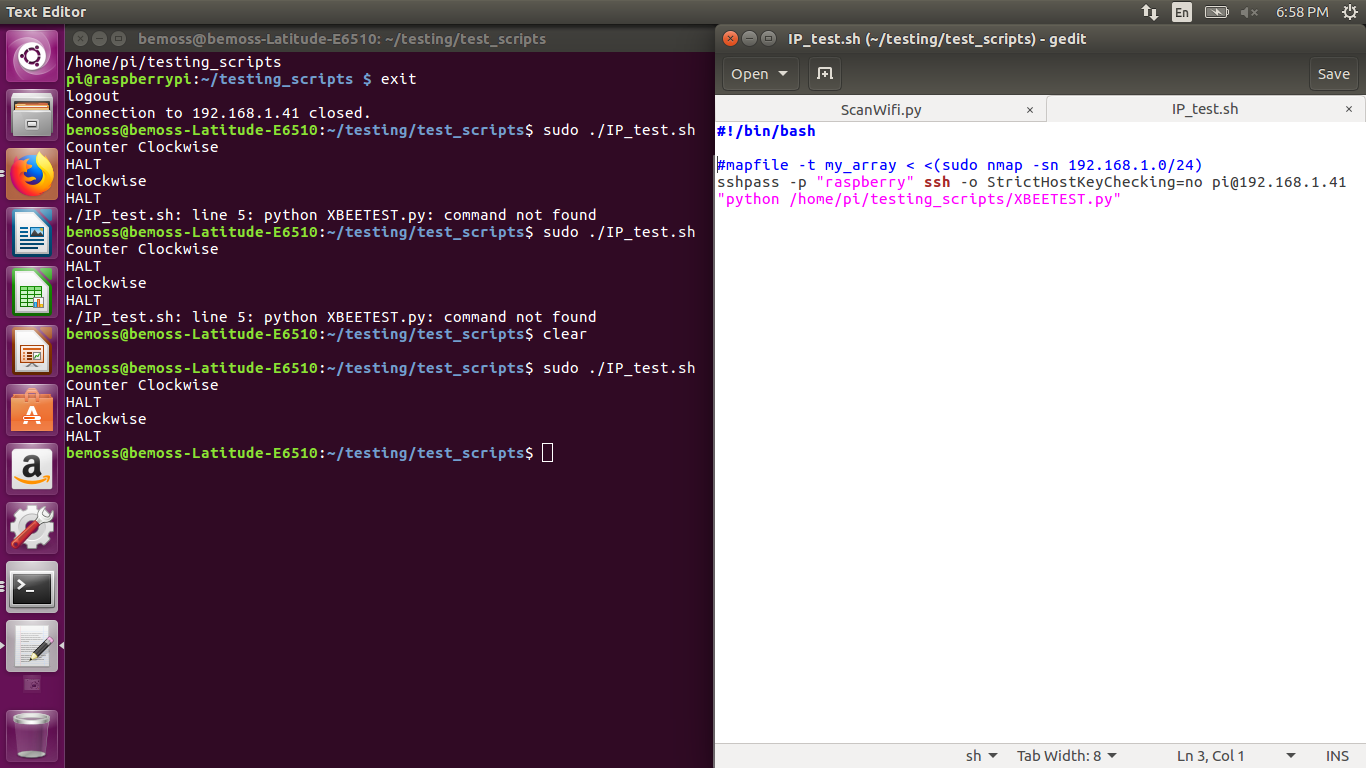
\includegraphics[width=1\textwidth]{figs/img/BashSSH.png}}
  \caption{Automatic SSH Bash code}
  \label{fig:BashSSH}
\end{figure}

In the figure "Automatic SSH Bash code", the bash script is shown along with the output in the terminal when it is is called. This script automatically sets up the ssh session to our IP address, inputs the password, and runs our script to transmit the motor commands over xbee. This script is very beneficial and can automate our entire process with a single function call. Our next step is to combine this with code to find all IP and MACs, comparing the MAC to our known RPI MAC format, and input the associated IP into this script. 

\labday{February 28, 2019}

Turn the bash script that we currently have into python code that is able to call the bash script that we currently have. Instead of hard coding the IP in, we should use the IP address that we find through the python script.
We also want to make it possible to push a button within BEMOSS and have our motor work properly.

To pass the IP and MAC variables found in our bash script to our python script, we plan to create a text file to drop them in and have referenced from our python scripts at a later time. Our "pyMAC identify" script will call the bash script to scan the network, place the variables in a text file, and sort through the text file to identify the RPI credentials from the list of found variables. From there, we will create a second text file that containsstrictly the credentials of every RPI on the network. This second text file will be opened and referenced by our "pyShellControl" script that will open up a ssh session with the RPI credentials found in the second text document. 

We succesfully created a text file from our bash script (called "MAC\_out.text" The next step will be to filter the results. 

\labday{March 5, 2019}
While working in the lab today, bob was able to successfully parse the text file that was created the other day and get the first instance of a raspberry pi on a network. A possible issue that is worth investigating is what the procedure will be if there are multiple raspberry pi's on the network. As of right now, the code only returns the first MAC address with the raspberry pi signature. If this becomes an issue, We will start looking into it but until then will continue moving forward and start using the found MAC address in our transmit code.

parse\_MAC.py is a script that compares all of the returned MAC addresses to that of the known characters in a Pi's MAC address. This works successfully. From here, we need to group an IP to that MAC address and automatically input it into our SSH connection script. 

Throwing Ideas down how to associate the IP:-------------
\begin{itemize}
    \item have the Pi return a certain thing when it is pinged?
    \item Filter out all words in the MAC\_out.txt to have raw IP and MAC data? 
    \item Any way to find out IP from MAC addr? (ARP looks to be the closest we get)
    \item  Brute SSH to every IP returned and try and input the credentials and see if we get in? (will utilize this method as a back up if more elegant ways aren't found) 
\end{itemize}
    
We are going to search for an EOL (end of line) character, create an indicie each time one is found and place the text found before the EOL character into that index. From there, we will use our MAC compare algorithm to find the indicie that matches. When we get a match, we will iterate 2 indexes up to where the associated IP is normally found. The output of this will be (hopefully) the associated IP 

SIDE NOTE: RASPBERRY PI PASSWORD CHANGED TO "BradleyEE" FOR SECURITY PURPOSES 

Update at 8:07 pm - we successfully iterated through our WiFi credentials text document titled "MAC\_out.txt". In this iteration, we found the MAC addr associated with a Raspberry PI. We then iterated two lines up to our IP addr line, iterated through this line's characters to the IP addr, and saved the IP addr to a variable. This iteration through the file is robust as it iterates through as many lines (Device credentials) that returned and the iteration through the IP line is robust as it can handle any size of IP addr. 

the next step is to pass the IP variable from our python iteration script to our Bash script that automates the SSH connection process. When these are combined, the total script will search for devices on the network, return all IPs and MACs, compare the MACs to that of a Raspberry PI, find the associated IP to that MAC, and input that IP into our connection process. 


END OF LAB DAY REPORT
all processes have been created and implemented (with exception of the IP variable being passed to the last script in fig RPI Identify). Reference the figure RPI Identify to see the process of how we identify a RPi and connect to it. This figure contains the names of scripts used, order of which they were used, which script each script calls, files that are created in each step, and files that are referenced in each step. 
\begin{figure}
  \boxed{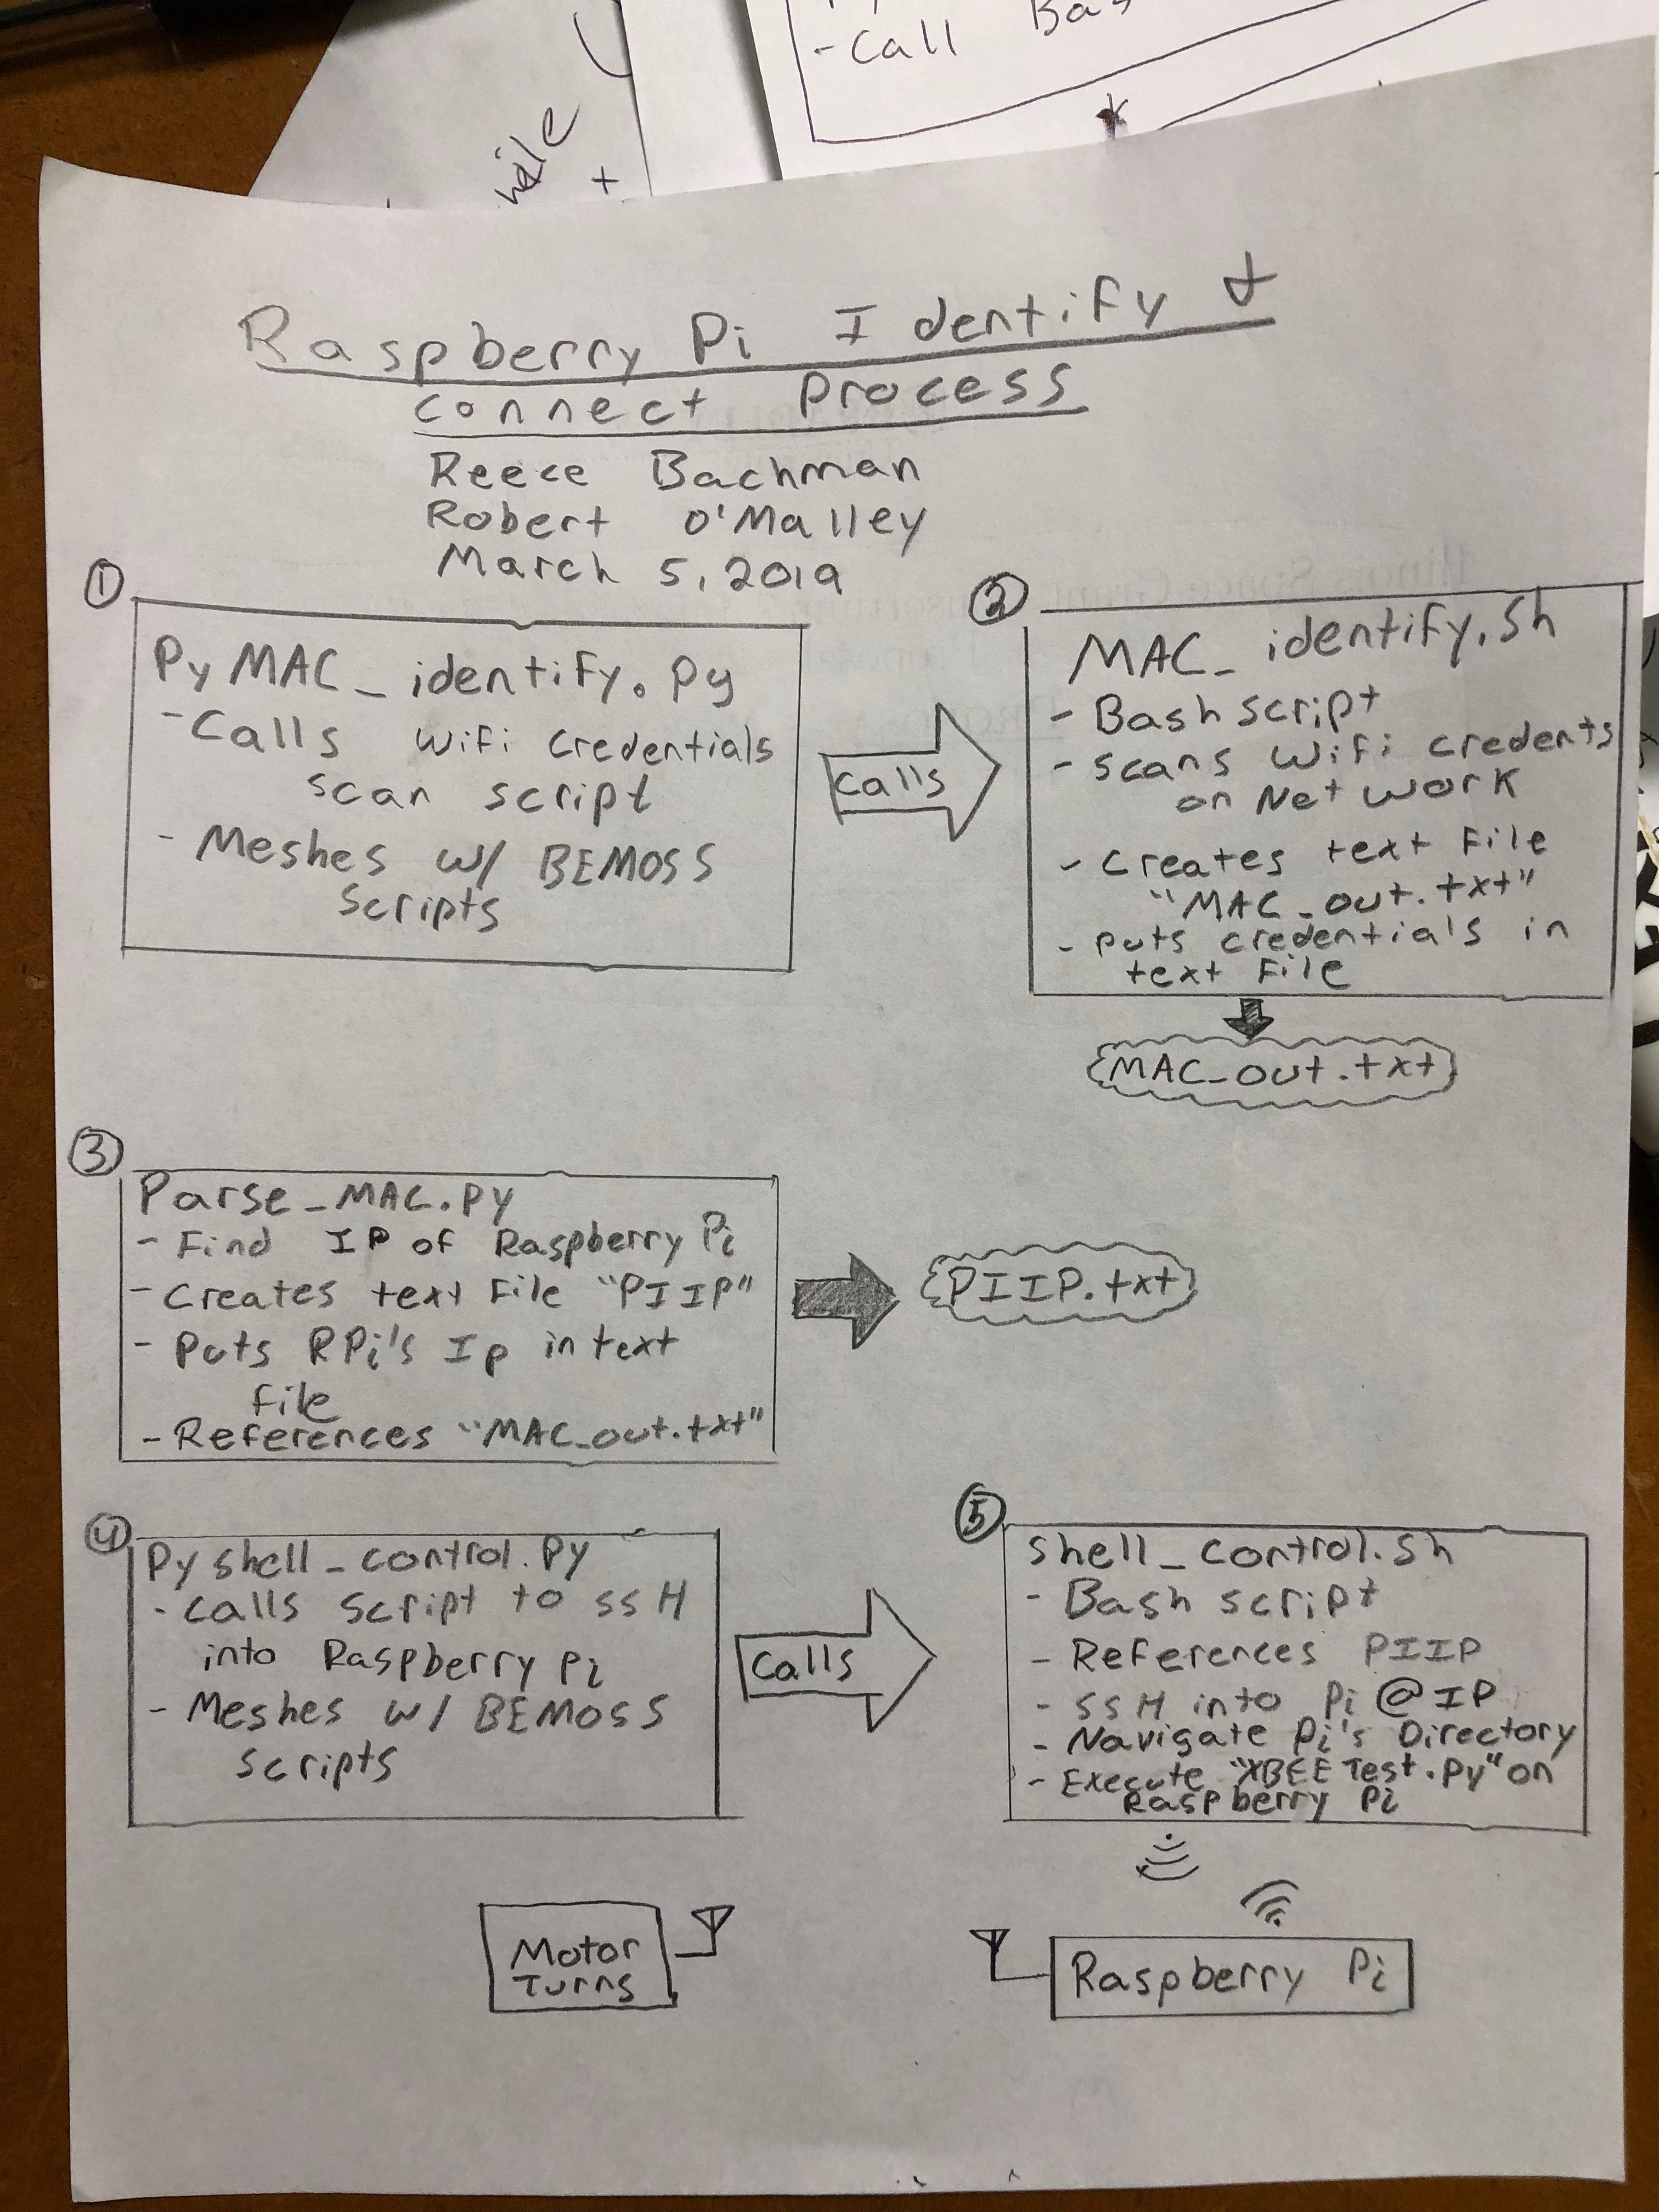
\includegraphics[width=1\textwidth]{figs/img/RPiIdent&Connect.jpg}}
  \caption{Raspberry Pi Identify and Connect Process}
  \label{fig:RPiIdentify}
\end{figure}

\labday{March 6}
Bob and Reece talk at 9 pm: Make a script on the laptop that automates the set up process for the raspberry pi. This script could 
\begin{itemize}
    \item Write the XBEE transmit script to a new Rpi over SSH 
    \item tell the pi which libraries (Xbee library, GPIO library, etc) to download to run the xbee transmit script
    
\end{itemize}

In theory, this makes our setup process very simple. All we would have to do is unbox the Rpi, give it a raspbian SD card, and connect it to the internet. 

From there, our script on the laptop will automatically find the Rpis on the network, SSH into them, make them download the proper libraries, transmit the XBEE code, and run them. 
\todo[inline]{This is very good. As you could figure out, there is much that can be used to improve the functionality of the existing  BEMOSS architecture. -- Dr. Miah}
    

\labday{March 8, 2019}
Reece will be working on the automation of the IP ssh
Bob will be working on the implementation of the hard coded version into BEMOSS
Jordan needs to set up a meeting with Professor Miah about the work with the model that has been done and the paper.
BEMOSS integration should be done before leaving for spring break
One more meeting next week
Talk with the team about moving our meeting to before 3
would like to set up a meeting with Ashraf before spring break

\labday{March 12, 2019}
To automate the process of finding and SSH into a Pi, 3 python scripts will need o be called: 
\begin{itemize}
    \item $pyMAC_identify.py$
    \item $parse_MAC.py$
    \item $pyshell.control.py$
\end{itemize}
I have thrown together a script that should automate which IP to SSH into based on the IP found in "PIIP.txt". This script is called shellconrolAuto. 
I (Reece) have no experience in bash. This will make the automation process very inefficient and timely to create. I can handle the logic and what needs to be exchanged between scripts to make the process work, but Bob's knowledge is needed. With Bob's help, the automation process will go much faster. 
\newline
WEEKLY MEETING
\newline
Bob is unsure on how to proceed with the GUI portion of BEMOSS. He will look into the GUI code from BEMOSS and try to develop a way to interface with the motor using a button. Bob will separate the python code that detects the IP addresses on the network and add the python code to the google drive. The current code requires administrator privileges to find the nearby devices, we can fix this problem at a later date to make it work without administrator privileges. Bob will also write a readme.txt file to explain the code to a new user. Also explain the current steps in the lab notebook. We will look into the code provided by BEMOSS's GUI code, may be able to click on the button and find it in the code. Otherwise we will search the code through matching the string from the GUI to the code.
\newline
Register the project for the student expo, the deadline to register is on Friday, March 15. We will work on the presentation for the expo to show all the hard work done by the group. Work on a catchy title to draw attention, come up with simple definition of IoT that still shows technical aspect. Dr. Miah will provide a template for the poster or we will use PowerPoint to create the poster. Use many figures and plots.
\newline
Try to implement the search aspect embedded in BEMOSS by Spring Break, this Friday. May have another meeting with Ashraf after Spring Break to help push the project to the end.
\newline
Wednesday at 2pm, Jordan and Dr. Miah will go over the paper to work on the mathematical model.


Looking through the html of BEMOSS, Bob was not able to find any helpful information within the html of BEMOSS as well as the GUI folder that is in BEMOSS.

\labday{March 13, 2019}

Jordan and Dr. Miah had a meeting today to discuss the research paper. To make progress we need to find the relative initial conditions of the system and use the LQR MATLAB code provided by Dr. Miah to create the K matrix. From there we can work backwards to find the control inputs. Further code will be updated in the shared Google Drive folder.

\labday{March 24, 2019}

Showing that we are able to run BEMOSS and determining some issues while trying to install it is a contribution. \#2 is running a piece of python code that scans all the access points and show all the mac and IP addresses. \#3 running python that shows mac and IP addresses which will send a command to 
no a and the on the poster board that we are making. We should have for the most part pictures. 
\begin{itemize}
    \item Professor Miah will be sharing the latex template with us for the poster
    \item We need to talk to Mr. Mattus about getting a router to use for the student expo as well as getting a new laptop
    \item We need to submit our abstract by April 3rd in Reece's email
    \item Try and have a test run in the Colosseum to show that our project can work there
\end{itemize}

piece of code on the computer separate from BEMOSS that will find the mac address, the IP addresses, and run the motor from the raspberry pi

\labday{April 2, 2019}

Bob has been working on finding the way to get a python script to run via html. When a check box is checked and a button is pushed, we should be able to run the python script that works our motor. right now looking at the onclick handler in html has given me a good basis to work with since this is my first time working in html.
\newline
Bob and Reece have been working on using his phone as a hotspot to connect to BEMOSS rather than a router for the expo.
\newline
Bob will continue to work on integrating the code onto BEMOSS. Ashraful has contacted the team to help finish the work sometime this week, through a Skype call. Bob needs to work on making the checkbox on BEMOSS's website to connect the motor. 
\newline
Reece will work to implement a GUI using Python to control the motor. He will start by programming two buttons, one for a clockwise direction and one for a counterclockwise direction. GUI should be complete by Thursday. Add GUI to pythonCode folder
\newline
For the expo we will focus on how we got BEMOSS to run and the challenges faced by it. If we cannot finish the GUI and integration for our motor by the expo we will show BEMOSS turning on and off and talk about turning on and off the motor using the shell scripting and talk about how we will implement the script into BEMOSS in the future.
\newline
The team needs to get the abstract done today and a rough draft of the report by Wednesday night. Send the abstract to Dr. Miah by tonight and the final report draft by Wednesday.
\newline
Jordan will use another method for solving the LQR system than the \cite{Khan2004}. TO simplify the case he will use the method from Dr. Miah's notes so as to not find $y_d^{(3)}$. The framework for the LQR method has been set up already and the rest of the work can be done soon. 


Reeces Gui:
So far I have this main script:


\begin{verbatim}
    

#CCWCWGui.py

import sys,os
from PyQt4 import QtGui, QtCore

#from CCWCWGui im
#import cwCall.py


#window = QtGui.QWidget()#window.setGeometry(50,50,500,300) #4 params: starting x, starting y, width, height, (0,0 top left) 


class Window (QtGui.QMainWindow):

	def __init__(self):
		super(Window,self).__init__()
		self.setGeometry(100,100,500,300)
		self.setWindowTitle("Rotation Direction")
		#self.ui=Ui_Form()
		#self.ui.setupUi(self)
		#self.ui.pushButton.clicked.connect(self.launch_script)
		

	def home(self):
		btn= QtGui.QPushButton("Close",self)
		btn.clicked.connect(QtCore.QcoreApplication.instance().quit)
		btn.resize(100,100)
		btn.move(100,100)

		#self.panel=cwCall.runscript()
		#self.panel.show()
		self.run()		
		self.show()




def run():
	app = QtGui.QApplication(sys.argv)
	GUI=Window()
	sys.exit(app.exec_())
run()
\end{verbatim}
This pops up a window thus far. I am working on creating a button that will close the window right now (as thats what the tutorials do first). I havent found a clear tutuorial on how to link these buttons to the python functions that shell to the py. I created individual scripts on the py to turn the motor clock wise and counter clockwise. To call these scripts over shell, I created python and bash scripts on the computer to call the rotation scripts individually. 

\labday{April 4, 2019}
Reece completed the GUI and it works as intended. I used Tkinter library and wrote the following code to produce 2 buttons:

\begin{verbatim}
    #!/usr/bin/env python
from Tkinter import *


master=Tk()
master.wm_title("Rotation")
master.geometry("300x260+500+50")


def clockwise():
	import subprocess
	subprocess.call("./cw.sh")

def ccw():
	import subprocess
	subprocess.call("./ccw.sh")
def closewindow():
	exit()

	



#CWbutton = Button(f, text="Clockwise", command=clockwise)

CWbutton=Button(master, text="Clockwise", command=clockwise, height=5, width=30)
CCWbutton=Button(master, text="Counter Clockwise", command=ccw, height=5, width=30)
close=Button(master, text="Close", command=closewindow, height=5, width=30)

CWbutton.pack()
CCWbutton.pack()
close.pack()

mainloop()



\end{verbatim}

GUI has 3 equally sized buttons: clockwise, counter clockwise, and close. 
%--------------- -----------------------------------------------------------------------
%	BIBLIOGRAPHY
%----------------------------------------------------------------------------------------


\labday{April 9, 2019}
Meeting with gave us information on what to be doing. He suggested that we might want to look at agent based architecture as opposed to just implementing a motor controller on a raspberry pi.
\begin{verbatim}
There should be three python files that should be able to do the following
1. get the device IP and MAC
2. get the current status with 1 or 0
3. control data, turn it on and off
'device_type_id': 2, 'api_name': '%CHANGE TO NAME OF FILE%'
consider proposing a new agent based architecture that could be implemented in BEMOSS
    
\end{verbatim}
These are the 3 python files that should be included. 
"We have disabled the linking between the searching and the controlling of our embedded computer as we have already linked it so that we can control it in front of you."

look into agent based architecture (different software than how bemoss works) 

For Poster:
\begin{itemize}
    \item Title: Change to BEMOSS:Building...Software
    \item Start with application and add figure similar to BEMOSS websites
    \item Next Objective, 
    \item Do not use A or The
    \item generalize when you can (i.e. embedded computer not raspberry pi)
    \item Don't need contributions at start
    \item Make picture similar to DOE picture, use only few colors with light background
    \item Use architecture from proposal with nice colors (Title: Proposed BEMOSS Architecture
    \item BEMOSS software architecture similar to on BEMOSS website
    \item Node detection needs figure showing how ubuntu is interfacing with a device. Wi-Fi symbol and RF symbol between server and items
    \item Control Algorithm: Include Simulink model as .PNG, put figure in fixed image folder. Experimental Results
    \item Also show Matlab results from Motor and House model on poster.
    \item Show GUI in experimental results
    \item Show BEMOSS running and screenshots from website
    \item Light bulb, plug switch, Router, Picture should be from straight shot, not angle. Use photoshop(GIMP is free) to add labels to devices 
    \item Two or three bullet points for future works.
    \item Email Draft of poster before noon tommorow. Afterwards email to Expo and Mattus
    \item Double check color choices to make sure it is easy to read.
    \item Start each point and total project with high level and work towards lower level.
    \item Bring Laptop, motor, light, router, other stuff ask Reece
\end{itemize}



\bibliographystyle{plain}
\bibliography{bib/seniorProject2017,bib/refsEnergy}

\labday{April 10, 2019}
Have the end of the arrow be outside of the picture and so the text box is outside of the picture.

In regards to the poster that we will be editing, Have application as the first heading and move the heading under it. Change the heading from BEMOSS to BEMOSS overview. Space in the title. BEMOSS overview should have the BEMOSS software architecture. Place objective and contribution that we have after the software architecture

Proposed BEMOSS architecture, Reece's IPE,  should be at the start for the second column. After that figure, new IoT configuration heading and the two pictures should be cropped better to not include the table. They should be subfigures. arrows need to be included for both of the pictures. Heading "Automatic detection and control". include EPS file instead of what we are using for figure 5.

Third column. "Second IoT device(HVAC)" is the heading we will use at the beginning of the third column. Move the dc motor model to the second column. Remove the "Control Algorithm" heading. Change the output of the data to a white background from simulink file. 

Fourth column. Mention that there is a menu that we do not have control of for the picture of BEMOSS. replace "future work" with "Summary and Future work". We need to make sure that our poster shows professionalism.


fig10. BEMOSS extracting data from l=plug load. need to talk about what each box is with arrow.


\labday{April 11, 2019}
Bob took time to get the three python scripts to work. As of right now, the first script works exactly as needs to for it to be implemented within BEMOSS. I also looked at django based web servers to try and get our script to work before adding the whole api.


\labday{April 16}

\begin{itemize}
\item  Integration done-bob
\item pwm drive-jordan 
  \begin{itemize}
  \item add PID control to the model 
  \item lqr model needs to be working 
  \end{itemize}
\end{itemize}



    
make what Reece has done for hardware and software easily relocatable (put it all in one spot) 
Bob make appendix for what he has done
Jordan makes appendix for what he has done 
30 pages for all of us combined 
appendices 

\labday{Arpil 18, 2019}
While in lab today, Bob was able to get the motor running through BEMOSS. the BEMOSS server is able to take a request from the user in the form of a URL and then the raspberry pi starts the motor. It is not a perfect version as right now there is not a button that will direct the user towards the page, so this needs to be changed soon. Adding a button to do so will involve some extra html studying. 
As stated above, right now the request is handled from the user entering a web page. It results in an ugly looking web page and a laggy interface. These will both be changed soon with a bit more studying of the django based server.

\todo[inline]{Great! Try to add the motor control button in BEMOSS so that it is prominent.} 

% \begin{thebibliography}{9}

% \bibitem{lamport94}
% Leslie Lamport,
% \emph{\LaTeX: A Document Preparation System}.
% Addison Wesley, Massachusetts,
% 2nd Edition,
% 1994.

% \end{thebibliography}

%----------------------------------------------------------------------------------------

\end{document}


%%% Local Variables:
%%% mode: latex
%%% TeX-master: t
%%% End:
